% SETUP
%----------------------------------------------------------------------------------------
% INITIAL CONFIG
%----------------------------------------------------------------------------------------

\documentclass[12pt,twoside]{report}


%----------------------------------------------------------------------------------------
% PACKAGES
%----------------------------------------------------------------------------------------

\usepackage{footnote}
%top=2cm, bottom=2cm, outer=1cm, inner=2.1cm, headsep=14pt
\usepackage[top=1.2in,bottom=1in,outer=0.8in,inner=1.2in,headsep=26pt]{geometry}          % For margins
\usepackage{graphicx}                        % For picture includes
\usepackage{xcolor}
\usepackage{float}                           % Used to set option H in figures
\usepackage{wrapfig}                         % To wrap figures with text
\usepackage{url}                             % URL in references
\usepackage{float}                           % For figure placing
\usepackage{amsfonts}                        % For fancy mathmode stuff (mathbb etc)
\usepackage{amsmath}                         % For useful math stuff like cases, align* etc
\usepackage{subcaption}                      % For subfigures and captions
\usepackage[parfill]{parskip}                % For new line instead of para indents
\usepackage{enumitem}                        % To do nested enumerations
\usepackage{verbatim}                        % Verbatim Output
\usepackage{microtype}                       % Improve spacing between words and letters
\usepackage{setspace}
\usepackage{booktabs}                        % Better looking tables
\usepackage{titlesec}                        % Formatting paragraphs as sections
\usepackage{fixltx2e}                        % Fixes some LaTeX stuff
\usepackage[colorlinks=false]{hyperref}       % Hyperlink References
\usepackage[capitalise]{cleveref}            % Clever Referencing
\usepackage{listings}                        % Code listings
\usepackage{longtable}                       % Don't break table across pages
\usepackage[british]{babel}                  % No idea
\usepackage{tabularx}
\usepackage{tikz}
%\usepackage[ruled, vlined, algoruled]{algorithm2e}
\usepackage{algorithm}
\usepackage{algpseudocode}
\usepackage{pgfplots}

\usepackage{fancyhdr}
\setlength{\headheight}{12pt}
\pagestyle{fancy}

% \RequirePackage[l2tabu, orthodox]{nag}       % Nags you if your syntax is wrong

%----------------------------------------------------------------------------------------
% TODOs
%----------------------------------------------------------------------------------------
\usepackage[colorinlistoftodos]{todonotes}
\setlength{\marginparwidth}{2cm}

%----------------------------------------------------------------------------------------
% QUOTING
%----------------------------------------------------------------------------------------
\usepackage{quoting}
\usepackage{csquotes}
\SetBlockEnvironment{quoting}% I've only added this

%----------------------------------------------------------------------------------------
% BIBLIOGRAPHY
%----------------------------------------------------------------------------------------
\usepackage[backend=bibtex,citestyle=authoryear,doi=true,url=true,urldate=long,sorting=none]{biblatex}
\setlength{\bibitemsep}{\baselineskip}
\addbibresource{references.bib}

%----------------------------------------------------------------------------------------
% BETTER TABLES
%----------------------------------------------------------------------------------------
\renewcommand{\arraystretch}{1.2}

%----------------------------------------------------------------------------------------
% FONT
%----------------------------------------------------------------------------------------
% \usepackage[sc]{mathpazo}
% \usepackage[T1]{fontenc}
% \linespread{1.05} % Palatino needs more leading (space between lines)


%----------------------------------------------------------------------------------------
% FRAMING FIGURES
%----------------------------------------------------------------------------------------

\floatstyle{boxed}
\restylefloat{figure}
% \restylefloat{table}

%----------------------------------------------------------------------------------------
% GLOSSARY
%----------------------------------------------------------------------------------------
\usepackage[toc,acronym]{glossaries}
\makeglossaries

%----------------------------------------------------------------------------------------
% CAPTIONS AND FIGURES
%----------------------------------------------------------------------------------------
% for figures: caption label is italic, the caption text is bold / italic
\captionsetup[figure]{singlelinecheck=on,justification=raggedright}

% for subfigures: caption label is bold, the caption text normal.
% justification is raggedright (i.e. left aligned)
% singlelinecheck=off means that the justification setting is used even when the caption is only a single line long. 
% if singlelinecheck=on, then caption is always centered when the caption is only one line.
\captionsetup[subfigure]{singlelinecheck=on,justification=raggedright}

%----------------------------------------------------------------------------------------
% IMPORTS
%----------------------------------------------------------------------------------------
%----------------------------------------------------------------------------------------
% USEFUL COMMANDS
%----------------------------------------------------------------------------------------


\newcommand{\ie}{i.\,e.}
\newcommand{\Ie}{I.\,e.}
\newcommand{\eg}{e.\,g.}
\newcommand{\Eg}{E.\,g.}

%----------------------------------------------------------------------------------------
% CODE LISTINGS SETUP
%----------------------------------------------------------------------------------------

\lstset{language=[LaTeX]Tex, % Specify the language for listings here
  keywordstyle=\color{RoyalBlue}, % Add \bfseries for bold
  basicstyle=\small\ttfamily, % Makes listings a smaller font size and a different font
  %identifierstyle=\color{NavyBlue}, % Color of text inside brackets
  commentstyle=\color{Green}\ttfamily, % Color of comments
  stringstyle=\rmfamily, % Font type to use for strings
  numbers=none, % Change left to none to remove line numbers
  numberstyle=\scriptsize, % Font size of the line numbers
  stepnumber=5, % Increment of line numbers
  numbersep=8pt, % Distance of line numbers from code listing
  showstringspaces=false, % Sets whether spaces in strings should appear underlined
  breaklines=true, % Force the code to stay in the confines of the listing box
  %frameround=ftff, % Uncomment for rounded frame
  frame=single, % Frame border - none/leftline/topline/bottomline/lines/single/shadowbox/L
  belowcaptionskip=.75\baselineskip % Space after the "Listing #: Desciption" text and the listing box
}

\lstdefinelanguage{JavaScript}{
  keywords={typeof, new, true, false, catch, function, return, null, catch, switch, var, if, in, while, do, else, case, break},
  keywordstyle=\color{blue}\bfseries,
  ndkeywords={class, export, boolean, throw, implements, import, this},
  ndkeywordstyle=\color{darkgray}\bfseries,
  identifierstyle=\color{black},
  sensitive=false,
  comment=[l]{//},
  morecomment=[s]{/*}{*/},
  commentstyle=\color{purple}\ttfamily,
  stringstyle=\color{red}\ttfamily,
  morestring=[b]',
  morestring=[b]"
}

\newacronym{RLE}{RLE}{Run Length Encoding}
\newacronym{KNN}{KNN}{K Nearest Neighbour}



% DOCUMENT
\begin{document}

\listoftodos

\onehalfspacing


\begin{titlepage}

\newcommand{\HRule}{\rule{\linewidth}{0.5mm}} % Defines a new command for the horizontal lines, change thickness here

\begin{center} % Center everything on the page

%----------------------------------------------------------------------------------------
% HEADING SECTIONS
%----------------------------------------------------------------------------------------


\includegraphics[width=0.3\textwidth]{gfx/icl-crest.jpg}

\textsc{\LARGE Imperial College London}\\[1.5cm] % Name of your university/college
\textsc{\Large MEng Individual Project}\\[0.5cm] % Major heading such as course name

%----------------------------------------------------------------------------------------
% TITLE SECTION
%----------------------------------------------------------------------------------------

\HRule \\[0.4cm]
{ \Large \bfseries Note\emph{Ed}}\\[0.4cm]
{ \large \bfseries An Interactive Manuscript Tutor for Fundamental Music Theory }\\[0.3cm]
\HRule \\[1.5cm]

%----------------------------------------------------------------------------------------
% AUTHOR SECTION
%----------------------------------------------------------------------------------------

\begin{minipage}{0.4\textwidth}
\begin{flushleft} \large
\emph{Author:}\\
Peter \textsc{Hamilton}
\end{flushleft}
\end{minipage}
~
\begin{minipage}{0.4\textwidth}
\begin{flushright} \large
\emph{Supervisor:} \\
Dr. Robert \textsc{Chatley}
\\[0.5cm]
\emph{Second Marker:} \\
Dr. Tony \textsc{Field}
\end{flushright}
\end{minipage}\\[4cm]

% If you don't want a supervisor, uncomment the two lines below and remove the section above
%\Large \emph{Author:}\\
%John \textsc{Smith}\\[3cm] % Your name

%----------------------------------------------------------------------------------------
% DATE SECTION
%----------------------------------------------------------------------------------------

{\large \today}\\[3cm] % Date, change the \today to a set date if you want to be precise

%----------------------------------------------------------------------------------------

\vfill % Fill the rest of the page with whitespace

\end{center}

\end{titlepage}

\chapter*{Abstract}
We would like to present Note\emph{ED} - an application which allows a child to practice their manuscript writing and music theory from home whilst receiving immediate feedback, outside of their music lessons.

In the course of the following dissertation we demonstrate that Note\emph{ED} is capable of recognising and analysing fundamental musical symbols both individually and in relation to each other and that it can do so in a way that enables useful feedback to a student in order to improve their written manuscript quality and reinforce concepts from fundamental music theory.

\todo[inline]{You can come up with a better abstract, just temporary}
\chapter*{Dedication}
\todo[inline,color=blue!30]{Add Dedication}
\chapter*{Declaration}
I declare that..
\chapter*{Acknowledgements}
\todo[inline,color=red]{Add Acknowledgements}

\begingroup
\hypersetup{linkcolor=black}
\tableofcontents
\endgroup

\pagebreak


\chapter{Introduction}

\section{Context}

Music is very old

\todo[inline,color=red]{Context - History of music teaching - top schools? Private vs Public?}
\todo[inline,color=red]{Context - Examine new forms of musical notation}
\todo[inline,color=red]{Context - Mention modern composers using things like Sibelius}
\todo[inline,color=red]{Context - Discuss children continuing to learn to write music the traditional way}
\newpage
\section{Motivation}

In the UK national curriculum for primary education, there is no requirement for children to learn to write or even read musical notation \parencite{Attai5}. However, when they're learning an instrument and reach the point where they need to take grades\footnote{ABRSM Subjects, Exams and Prerequisites \url{http://gb.abrsm.org/en/our-exams/information-and-regulations/}}, this is something they must be able to do \parencite{whyMusicTheory}.

Learning to write musical manuscript correctly and clearly takes time and practice, much as when children are learning normal handwriting skills. From informal research it is clear that most instrumental teachers would like their pupils to learn written music theory alongside their practical instrumental tuition.

However there often isn't an abundance of time to spend on learning and practicing music theory and so the options available to the student and teacher are therefore limited. Do you go over the topic during lesson time, eating into the instrumental tuition, or do you perhaps sending the child away with some manuscript paper\footnote{An example of blank manuscript paper can be found at \url{http://www.blanksheetmusic.net/}} and `homework', which can be marked during their next lesson, using yet more time. Sadly both of these are often ineffective methods of learning since without guidance and feedback on a regular basis, it's all too easy for a student to accidentally reinforce bad habits, \textbf{A faster, unsupervised feedback loop} is needed.

Whilst several solutions exist that can help children with academic theory as we can see in \cref{sec:music-theory-apps}, the subject of handling handwritten notation and manuscript has so far not been tackled. \textbf{\acrfull{OMR}} is a field I draw on heavily in this dissertation. Commericial and research applications in this area typically focus on converting draft or rough handwritten notation into a digital format and are not primarily educational tools. With such tools, no feedback is provided and indeed extracting feedback would be hard given the technical methods used to analyse the musical scores.

In short, \textbf{no application exists which is capable of helping a child learn to correctly write musical notation whilst simultaneously providing feedback} other than their music teacher. This project aims to make a start towards filling that void.
\newpage
\section{Objectives}

\subsection*{Image Analysis}
Build a service which is capable of analysing a notation drawing and establishing one or more scores for multiple aspects of a notation attempt based on a reference example and/or previous attempts.

\subsection*{Tablet Interface}
A tablet oriented (or tablet compatible) user interface which can provide a child with simulated challenges around writing musical notation and easily allow them to input their attempts and display feedback.

\subsection*{Engaging Experience For Child}
Combine the two objectives above to produce a streamlined experience which a child will happily engage with on a repeat basis

\subsection*{Learning Improvement}
Produce a application which improves on and encourages a child's learning outside of lessons


\chapter{Background}

\section{Manuscript Basics}

\blockquote{``Right from the start, it is important to learn how to write down music clearly. As a musician, unclear manuscript can waste valuable rehearsal time and might lead to performance mistakes. In an exam, badly written work may be misunderstood and could lose you vital marks.'' \cite{taylor1989ab}}


For early grades of music theory, the criteria by which students need to adhere in order to maximize their marks and musical potential is covered in quite specific detail. This makes sense as the majority of students taking the exam are likely to be young and since they are also unlikely to have encountered much written music before, this is the most crucial time for teaching them good habits.

I will attempt to give a walk through of the basic manuscript entities that a student aiming to take their grade 1 - 3 theory exams would most likely have to know about and/or write down, along with the relevant criteria for what constitutes acceptable and unacceptable manuscript, mostly examples below are taken from or based on the official documentation in \cite{taylor2008music}


\subsection*{Notes on the stave}

\subsubsection*{Semibreve}

The semibreve is the easiest note to draw and is simply an oval outline, however, the rules which govern it's placement are quite specific as outlined in Figures \ref{fig:SemibreveOnLine} \& \ref{fig:SemibreveOnSpace}

\begin{figure}[h!]
  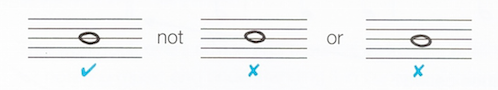
\includegraphics[width=\linewidth]{gfx/basic/semibreve-on-line.png}
  \centering
  \caption{If it is drawn on the line, the line must go exactly through the middle of the semibreve}
  \label{fig:SemibreveOnLine}
\end{figure}

\begin{figure}[h!]
  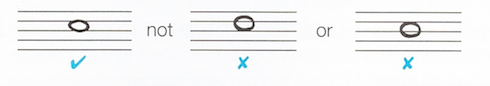
\includegraphics[width=\linewidth]{gfx/basic/semibreve-on-space.png}
  \centering
  \caption{If it is drawn in the space, it should also only cover half the space on either side}
  \label{fig:SemibreveOnSpace}
\end{figure}

\subsubsection*{Ledger Lines}

Notes can be drawn higher or lower than the five stave lines by drawing another line or lines above or below the stave.

\begin{figure}[h!]
  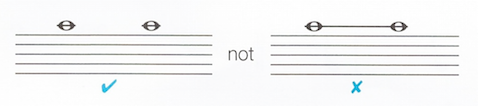
\includegraphics[width=\linewidth]{gfx/basic/ledger-boundaries.png}
  \centering
  \caption{Each note must have it's own line restricted to the boundaries of the note}
  \label{fig:LedgerBoundaries}
\end{figure}


\begin{figure}[h!]
  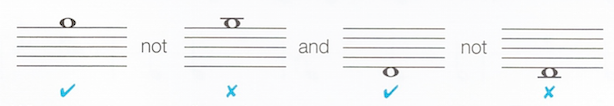
\includegraphics[width=\linewidth]{gfx/basic/ledger-above.png}
  \centering
  \caption{Lines should not be drawn over notes just above the stave, or below a note just under the stave}
  \label{fig:LedgerAbove}
\end{figure}


\begin{figure}[h!]
  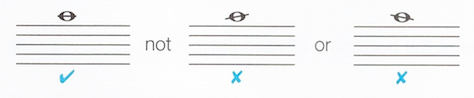
\includegraphics[width=\linewidth]{gfx/basic/ledger-slope.png}
  \centering
  \caption{The lines you draw through notes should not slope up or down, but should be exactly horizontal}
  \label{fig:LedgerSlope}
\end{figure}

\subsection*{Stems}

The stem of a note should go up on the right and down on the left. Which version to use depends on which line the head of the note is placed upon.

The stems of the notes on the top two lines should go down
The stems of the notes on the bottom two lines should go up
The stems of the notes on the middle line can go either up \emph{or} down.

\begin{figure}[h!]
  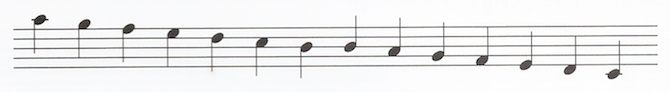
\includegraphics[width=\linewidth]{gfx/basic/stems-chromatic.png}
  \centering
  \caption{Examples of note stem direction}
  \label{fig:StemsChromatic}
\end{figure}

How the stems are drawn is quite important as they must not be too long or too short and should be vertically straight.

\begin{figure}[h!]
  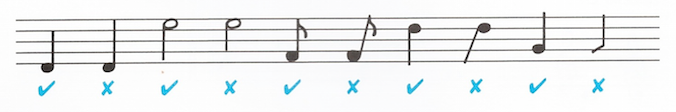
\includegraphics[width=\linewidth]{gfx/basic/stems-good-bad.png}
  \centering
  \caption{Examples of good and badly drawn note stems}
  \label{fig:StemsGoodBad}
\end{figure}

Quavers and eighth notes have small tails on them, typically in printed music they're curved but for handwritten notation straight lines are perfectly acceptable.

\begin{figure}[h!]
  
\includegraphics[width=0.4\linewidth]{gfx/basic/stems-curved.png}
  \centering
  \caption{Examples of straight and curved note stems}
  \label{fig:StemsStraightCurved}
\end{figure}

\subsection*{Clefs}

\subsubsection*{Treble Cleff}

The treble clef is one of the more difficult symbols to master, but has a fairly straightforward technique. You start with a loop around the \emph{G} line (second from the bottom) and then follow through with the loops.

\begin{figure}[h!]
  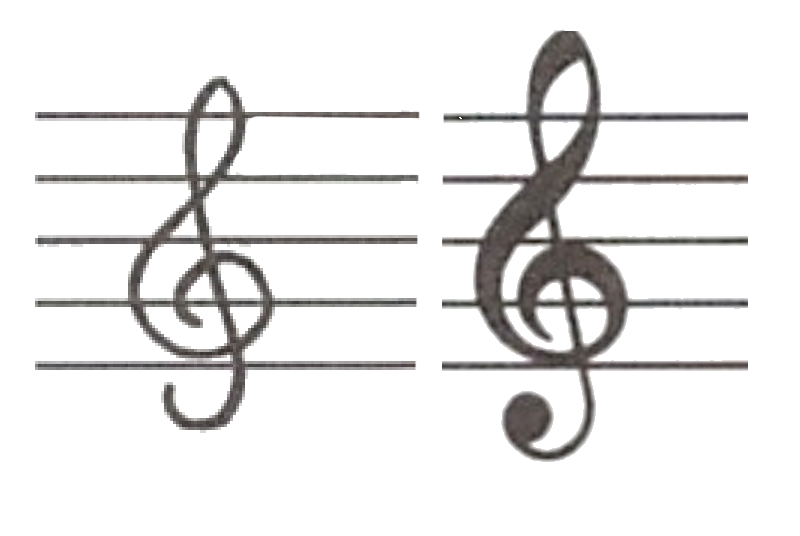
\includegraphics[width=0.3\linewidth]{gfx/basic/treble-clef.png}
  \centering
  \label{fig:TrebleClef}
\end{figure}

\subsubsection*{Bass Clef}

The bass clef has two different variations, both with two dots to the right, either side of the \emph{F} line (second from the top) around which the core of the clef is centered. The left variation is by far the most common.

\begin{figure}[h!]
  
\includegraphics[width=0.5\linewidth]{gfx/basic/bass-clef.png}
  \centering
  \caption{Two versions of the Bass Clef}
  \label{fig:BassClef}
\end{figure}

\subsection*{Beaming}

Notes with tails are often joined together, known as \emph{beaming}. For example, you can beam the following notes together:

\begin{figure}[h!]
  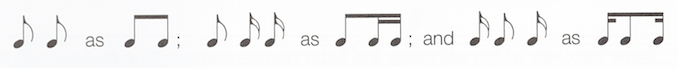
\includegraphics[width=\linewidth]{gfx/basic/beaming.png}
  \centering
  \caption{Notes and their beamed equivalents}
  \label{fig:NotesBeamedEquiv}
\end{figure}


\subsection*{Rests}

\begin{enumerate}
\item The semibreve rest hangs below a line (usually the fourth) and is depicted by a rectangle which fills half the line space.
\item The minim rest is depicted similarly, but above the line (usually the third)
\end{enumerate}

\begin{figure}[h!]
  
\includegraphics[width=0.7\linewidth]{gfx/basic/semibreve-minim-rest.png}
  \centering
  \caption{Examples of the semibreve rest (left) and minim rest (right)}
  \label{fig:RestMinimSemibreve}
\end{figure}

You can draw a crochet one of two ways and although the first is harder to draw, it is the most commonly used, so is the preferred version when learning to write music. This, and examples of a quaver and semiquaver rest can be seen in Figure \ref{fig:RestCrochetQS}

\begin{figure}[h!]
  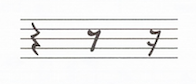
\includegraphics[width=0.5\linewidth]{gfx/basic/rests.png}
  \centering
  \caption{Examples of crochet, quaver and semiquaver rests}
  \label{fig:RestCrochetQS}
\end{figure}

\subsection* {Ties}

A tie joins notes which sound the same and turns them into one sound. For example:

\begin{figure}[h!]
  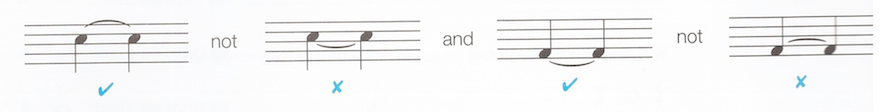
\includegraphics[width=\linewidth]{gfx/basic/ties.png}
  \centering
  \caption{Example of tied notes}
  \label{fig:TiedNotes}
\end{figure}

You can join any number of notes in this way, but they must be the same notes and they must be next to each other, the tie goes from the head of the first note to the head of the next.

\subsection*{Dotted Notes}

Dotted notes are very simple to draw and their purpose is even simpler. They make any dotted note equal to 1.5 $\times$ the length of the same note without the dot.

\begin{figure}[h!]
  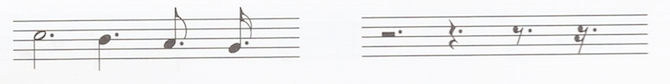
\includegraphics[width=\linewidth]{gfx/basic/dotted-notes.png}
  \centering
  \caption{Dotted Notes}
  \label{fig:DottedNotes}
\end{figure}

\subsection*{Accidentals}

When placed on staff lines or spaces, accidentals modify the note which they precede. They must lie evenly across a line or a space because as with previous notation, bad placement leads to ambiguity an lost marks

\begin{enumerate}
\item Sharps modify a note by adding a semitone to it's original value
\item Flats modify a note by subtracting a semitone to it's original value
\item Naturals modify a note by removing the influence of any previous sharps or flats.
\end{enumerate}

\begin{figure}[h!]
  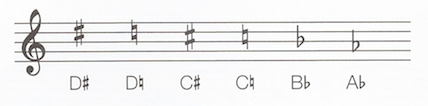
\includegraphics[width=\linewidth]{gfx/basic/accidentals.png}
  \centering
  \caption{Examples of accidentals}
  \label{fig:Accidentals}
\end{figure}



\section{Existing OMR Applications}

Prior to embarking on a solution from scratch, an understanding of the existing OMR landscape and whether any tools already existed was done. Several software solutions were found which can help someone take a printed score (or even an older handwritten one) and process it to create a digital representation. However, the majority were commercial applications which required purchasing and almost were designed to be used under highly supervised conditions, doing an initial conversion and then guiding the user through the process of validating the applications `best guess'.

\subsection{Neuratron Photoscore}
Neuratron Photoscore\footnote{http://www.neuratron.com/photoscore.htm} is one of the market leading packages, features tight integration with several composition tools like Sibelius and Finale, outputs to a range of formats (MusicXML etc). Designed to be run by the end user in supervised conditions, going over a scanned sheet and correcting errors as you go

\subsection{Audiveris}
``Audiveris is an open-source Optical Music Recognition software which processes the image of a music sheet to automatically provide symbolic music information in MusicXML standard.''\footnote{https://audiveris.kenai.com/}
\newline
At present it only supports high quality printed scores and operates by utilising a neural network which must be trained on samples by the end user.

\subsection{Gamera}
Gamera\footnote{http://gamera.informatik.hsnr.de} is primarily a structured document processing and symbol recognition tool \parencite{macmillan2002gamera} and was spun out of one of the authors' previous thesis which focussed on OMR \parencite{fujinaga1996adaptive}. Primarily used for academic purposes, it has some great projects, one of which specialises in supporting research into stave detection and removal \footnote{http://gamera.informatik.hsnr.de/addons/musicstaves/}.

\subsection{Capella Scan}
As with most of the other applications mentioned, Capella Scan\footnote{http://www.capella.de/us/index.cfm/products/capella-scan/info-capella-scan/} is primarily designed to convert old or dated music manuscripts into a more ``preservable'' digital format without needing to manually type all the music out again

\section{Music Theory Applications}
A search online and of the Apple ``App Store'' revealed several examples of applications which teach music theory, however none of these focus on writing music and are more based around ideas like flashcards and memorisation.

\begin{figure}[h!]
  \centering
  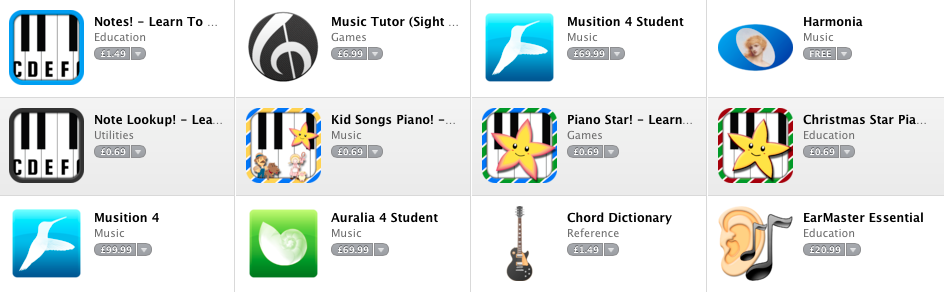
\includegraphics[width=\linewidth]{gfx/music-theory-apps.png}
  \caption{Music Theory Applications after searching ``Music Theory'' on the Apple App Store}
\end{figure}

Most of these apps however, are aimed at more advanced students and miss out a huge part of theory exams which is the written notation section.

\section{Music Theory Workbooks}

\chapter{Technical Research}

\section{Previous Works}
\subsection{\cite{taubman2005musichand}}
\label{sec:domain-knowledge-taubman}
In this paper, Taubman attempts to improve on notation input for professional musicians, allowing them to input rough ``sketched'' music and convert it into a neatly printed form. The application created, ``MusicHand'' makes use of a graphics tablet connected to a desktop machine and records the individual strokes the user makes.

Strokes are captured individually but using a latency threshold which is then used to group the strokes together, adjusted on a per user basis. Taubman then makes use of statistical moments \todo[inline]{Reference to Moments Tech background} to classify these stroke groups, then making use of a K-NN algorithm to classify the object as one of several musical entities using the generated moments.

\begin{figure}[H]
  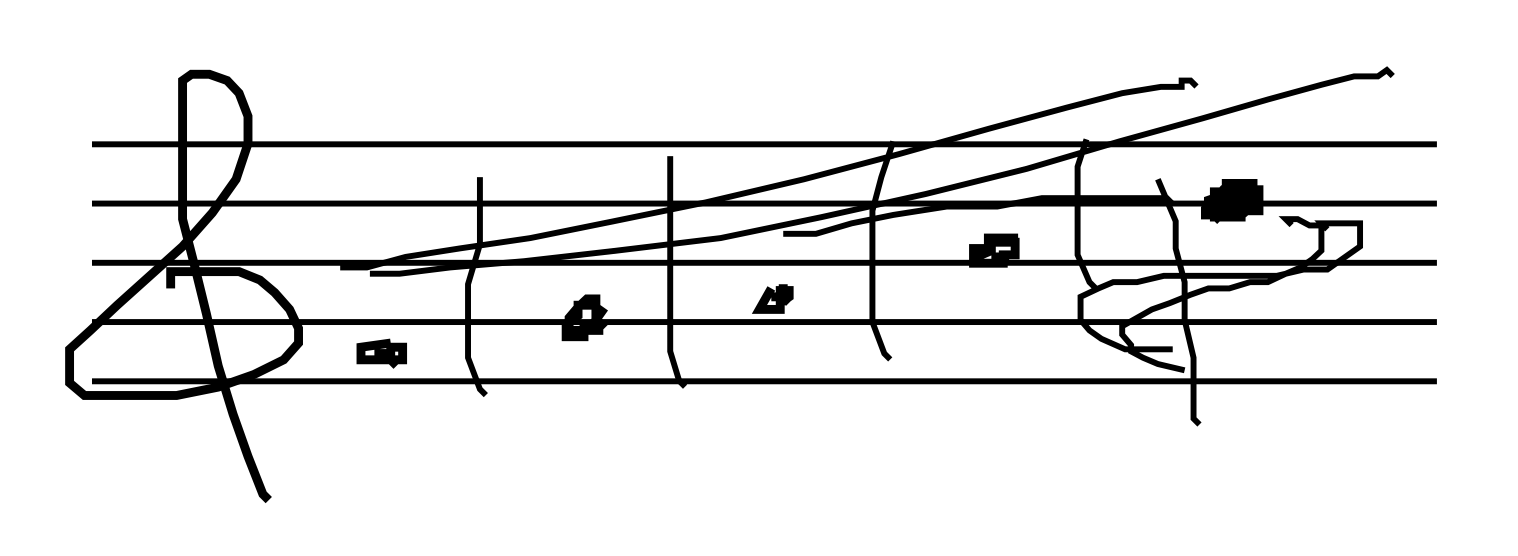
\includegraphics[width=\linewidth/2]{gfx/prior-research/taubman-sketch.png}
  \centering
  \caption{Example notation sketch from \cite{taubman2005musichand}}
  \label{fig:taubman-sketch}
\end{figure}

Since strokes are generally sketched as seen in \cref{fig:taubman-sketch} the application also makes use of a great deal of domain expertise, covered further in \cref{sec:domain-expertise}, essentially running through a large flow chart in order to classify the entities further. However, the system notably relies on the compatibility of the generated moment ``libraries'' between users, a study of which was recommended for any future work but not done in this case. It is also suggested that instead of a graphics tablet, one might experiment with a more direct input method such as drawing onto a tablet directly with a stylus, the author specifically mentions the ``Wacom Cintiq''\footnote{http://uk.shop.wacom.eu/products/cintiq}, a ``digital canvas'' of sorts, which might allow a much more natural pen-paper feel.


\subsection{\cite{george2003online}}
\todo[inline,color=red]{Technical Background - Summarise George Paper}

\subsection{\cite{fujinaga1996adaptive}}

Fujinaga's thesis proposed an adaptive system for use with OMR etc

Fujinaga's technique involves the seperation of musical elements from the staves, followed by
classification using a \acrfull{KNN} classifier. He proposes several features for use in classification including \todo[inline]{What features does fujinaga use?}

\todo[inline,color=red]{Technical Background - Summarise Fujinaga Paper}

\subsection{\cite{benoptical}}

An interesting component of the work by Ben-Dayan and Giloh was their experiments with stem, note head and symbol detection during the segmentation phases.

\subsubsection{Stem Detection}

For stem detection, since handwritten stems are unlikely to be perfectly straight, the authors use vertical projections combined with a high pass filter to establish likely stems. These are represented by peaks in the vertical projection.

A bounding box is then generated and the note is split into an upper and lower region; the upper and lower parts being used in note head and beam detection later.

\subsubsection{Note Head and Features Detection}

The author extracts the head position by way of a distances transform and then examining the density of the pixels (distance from the nearest black pixel) the results of which you can see graphically in \cref{fig:giloh-component-centre}. The authors also make several assumptions at this stage regarding the size of features (e.g. sharps are less than twice the stave space height) which enables them to separate notes from other components (clefs, accidentals etc).

\begin{figure}[H]
  \centering
  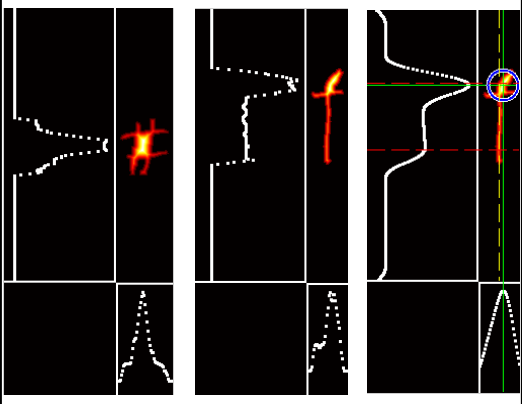
\includegraphics{gfx/prior-research/giloh-component-centre}
  \caption{Finding component centres, \parencite{benoptical}}
  \label{fig:giloh-component-centre}
\end{figure}



\section{Generating Manuscripts}

In order to produce enough musical examples and references for a student to use, some automated way of producing the reference manuscript is  needed.

\subsection{Professional GUI Tools}
\label{sec:ProfTools}
There are several professional tools which are used in industry to generate musical scores on the computer. The ones with most widespread usage are Sibelius\footnote{http://www.avid.com/US/products/SibeliusFirst/overview} and Finale\footnote{http://www.finalemusic.com/products/finale/} and more recently, NoteFlight\footnote{http://www.noteflight.com/}

They're worth mentioning as they're the ``industry standards'' for musical notation and composition, used by professionals and in education around the world, but their primary use case is manual input via a GUI so for our purposes they are not ideal.

\subsection{LilyPond}
\label{sec:lilypond}

LilyPond\footnote{http://www.lilypond.org/} is a music engraver and serves as a \enquote{modular, extensible and programmable compiler for producing high-quality music notation} \parencite{nienhuys2003lilypond}. Originally inspired by the efforts of projects like MusixTex\footnote{http://www.mab.jpn.org/musictex/musixtex\_e.html} which had aimed to \enquote{be able to typeset complex polyphonic, orchestral or instrumental music} \parencite{Taupin99musixtex–using} in the same way that it was already renowned for beautifully typeset text and maths. It's a widely adopted tool but it's flexibility with regard to formatting made it difficult to learn.

The idea of Lilypond was that by entering or programmatically generating a formal representation of music which is designed to be easy to type, you can then use LilyPond to produce a manuscript engraving form that representation. They also support conversion from other popular text-based music formats such as MusicXML\footnote{Some good examples can be found at http://www.musicxml.com/tutorial/hello-world/}, or ABC\footnote{Standards can be found at http://abcnotation.com/}.

For example, given the following LilyPond syntax:

\begin{lstlisting}
\relative c' {
  c' d' e' f' g'2 g'2
}
\end{lstlisting}

We can run LilyPond to produce the output you see in figure \ref{fig:lilypond-output}

\begin{figure}[h!]
  
\includegraphics[width=\linewidth]{gfx/background/lilypond-output.png}
  \centering
  \caption{Lilypond Output Example}
  \label{fig:lilypond-output}
\end{figure}

Using Lilypond and some basic algorithms around music theory we could easily generate textual representations of exercises and generate the necessary images from them. It's also free and accessible meaning that I can easily install it on development machines and servers.

\subsection{VexFlow}

Vexflow\footnote{https://github.com/0xfe/vexflow} is another music engraving application, but Vexflow is web based and makes use of HTML5 Canvas\footnote{https://developer.mozilla.org/en/docs/HTML/Canvas} and SVG\footnote{http://en.wikipedia.org/wiki/Scalable\_Vector\_Graphics} so it can be used to generate manuscripts on the fly in a browser.

For example if you were to include the vexflow library and then write the javascript outlined in \ref{lst:vexflow} you will get the result in figure \ref{fig:vexflow-output}

\begin{figure}[h!]
  \begin{lstlisting}[language=JavaScript]
  var canvas = $("div.one div.a canvas")[0];
  var renderer = new Vex.Flow.Renderer(canvas,
    Vex.Flow.Renderer.Backends.CANVAS);

  var ctx = renderer.getContext();
  var stave = new Vex.Flow.Stave(10, 0, 500);
  stave.addClef("treble").setContext(ctx).draw();
  \end{lstlisting}
  \label{lst:vexflow}
\end{figure}

\begin{figure}[h!]
  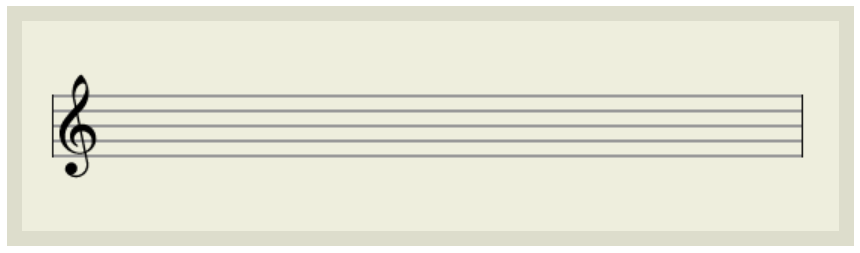
\includegraphics[width=\linewidth]{gfx/vexflow.png}
  \centering
  \caption{Vexflow render, see \url{http://vexflow.com/docs/tutorial.html}}
  \label{fig:vexflow-output}
\end{figure}

An advantage vexflow has over \nameref{sec:lilypond} is that for use on the web, we would need to render the music remotely on the server with lilypond, then synchronously or asynchronously transport those resources (most likely images, which are expensive for web traffic) to the client. The downside of client side rendering is of course that for anything complex, since it increases the load on the end device, it's important to be aware on which devices the code will primarily be run to ensure a good user experience.



\section{OMR Architecture}

In general, the challenge of OMR can be decomposed into more defined sections. Although implementations obviously differ, an overview of some of the techniques I have come across for the various `common' stages which I researched can be summarised by:

\begin{table}[H]
  \footnotesize
  \begin{tabularx}{\linewidth}{ X X X X }
    \toprule
    \textbf{1. Pre Processing} & \textbf{2. Segmentation} & \textbf{3. Classification} &  \textbf{4. Reconstruction} \\
    \midrule

    \begin{enumerate}[leftmargin=*]
      \item Level Adjustment
      \item Binarization
      \item Noise Removal
      \item Handling Skew
      \item Rotation
      \item Stave Removal
        \begin{enumerate}
          \item Horizontal Projections
          \item Hough Transforms
        \end{enumerate}
    \end{enumerate}

    &

    \begin{enumerate}[leftmargin=*]
      \item Projections
      \item Template Matching
      \item Connected Components
    \end{enumerate}

    &

    \begin{enumerate}[leftmargin=*]
      \item \acrfull{KNN}
      \item Neural Networks
      \item Support Vector Machines
      \item Statistical Moments
    \end{enumerate}

    &

    \begin{enumerate}[leftmargin=*]
      \item Simple Heuristics
      \item Grammar
    \end{enumerate} \\
    \bottomrule
  \end{tabularx}

  \caption{Typical OMR Stages}
  \label{table:omr-stages-typical}
\end{table}

\section{Segmentation}

Segmentation is the challenge of taking a given image or scene and extracting individual objects or `components'.

Typically this can be a complex problem to tackle as stafflines connect almost all components together and must therefore first be removed. Also some musical entities are themselves comprised of multiple other entities. Good examples are the bass clef which is comprised of two dots placed above each other to the right of the curve and dotted notes , both of which can be seen in \todo[inline]{Examples of multi-component musical entities}.

Particularly in this project, we also need to be able to break down the musical entities further into stems and note heads and so separating these from each other present another problem which we must take into account.

\subsection{Connected Component Analysis}

Connected component analysis is a technique used to establish distinct regions within an image. An individual pixel in a binary image can possess two forms of connectedness, \emph{4-neighbour} or \emph{8-neighbour}. It should be noted that this evaluation only takes place for pixels with a value of 1 or ``filled pixels''.

More formally, ``A connected component labelling of a binary image B is a labeled image LB in which the value of each pixel is the label of it's connected component'' \parencite[pg 69]{shapiro2001computer}

To be \textbf{4-neighbour}, at least one of the pixels above, below or to the left or right (which we can refer to as the vertical and horizontal neighbours) of the pixel under investigation must have a value of 1.

In a similar fashion, an \textbf{8-neighbour} pixel is one where any of the surrounding 8 pixels (vertical, horizontal or diagonal neighbours) has a value of 1.

Regions for 4-neighbour and 8-neighbour connected pixels are outlined in figure \ref{fig:pixel-neighbours}

\begin{figure}[h!]
  \centering
  \subfigure[4 Neighbour Regions]{
    \begin{tikzpicture}
  \fill[green!60] (1,1) rectangle (2,2);
  \fill[gray!60]  (1,0) rectangle (2,1);
  \fill[gray!60]  (0,1) rectangle (1,2);
  \fill[gray!60]  (2,1) rectangle (3,2);
  \fill[gray!60]  (1,2) rectangle (2,3);
  \draw[thick,step=1cm,color=gray!30] (-1, 0) grid (4,3);
\end{tikzpicture}

    \label{fig:4-neighbour-regions}
  }
  \quad
  \subfigure[4N - 2 Regions Identified]{
    \begin{tikzpicture}
  \fill[red]      (1,1) rectangle (2,2);
  \fill[gray!60]  (1,0) rectangle (2,1);
  \fill[gray!60]  (0,1) rectangle (1,2);
  \fill[red]      (2,1) rectangle (3,2);
  \fill[gray!60]  (1,2) rectangle (2,3);
  \fill[blue]     (2,2) rectangle (3,3);
  \draw[thick,step=1cm,color=gray!30] (-1, 0) grid (4,3);
\end{tikzpicture}

    \label{fig:4-neighbour-connected}
  }\\
  \subfigure[8 Neighbour Regions]{
    \begin{tikzpicture}
  \fill[green!60] (1,1) rectangle (2,2);

  \fill[gray!60]  (0,0) rectangle (1,1);
  \fill[gray!60]  (1,0) rectangle (2,1);
  \fill[gray!60]  (2,0) rectangle (3,1);

  \fill[gray!60]  (0,1) rectangle (1,2);
  \fill[gray!60]  (2,1) rectangle (3,2);

  \fill[gray!60]  (0,2) rectangle (1,3);
  \fill[gray!60]  (1,2) rectangle (2,3);
  \fill[gray!60]  (2,2) rectangle (3,3);
  \draw[thick,step=1cm,color=gray!30] (-1, 0) grid (4,3);
\end{tikzpicture}

    \label{fig:8-neighbour-regions}
  }
  \quad
  \subfigure[8N - 1 Region Identified]{
    \begin{tikzpicture}
  \fill[red]   (1,1) rectangle (2,2);

  \fill[gray!60]  (0,0) rectangle (1,1);
  \fill[gray!60]  (1,0) rectangle (2,1);
  \fill[gray!60]  (2,0) rectangle (3,1);

  \fill[gray!60]  (0,1) rectangle (1,2);
  \fill[red]      (2,1) rectangle (3,2);

  \fill[gray!60]  (0,2) rectangle (1,3);
  \fill[gray!60]  (1,2) rectangle (2,3);
  \fill[red]      (2,2) rectangle (3,3);
  \draw[thick,step=1cm,color=gray!30] (-1, 0) grid (4,3);
\end{tikzpicture}

    \label{fig:8-neighbour-connected}
  }

  \caption{4 and 8 Neighbour Regions and examples of connected pixels}
  \label{fig:pixel-neighbours}
\end{figure}

There are two primary algorithms for establishing connected regions, the first is recursive and the second requires two scans.

\subsubsection{Recursive Labelling}

If we assume that the size of the image to be evaluated is small and we can fit it in memory (a reasonable assumption give the scope of the project and the hardware available) we can employ a recursive algorithm which can grow regions by visiting any pixel in the image using depth first of breadth first searching. An outline for a depth first algorithm is given in algorithm \ref{alg:ccl-recursive}

% \begin{algorithm}[ht]
%   \SetKwFunction{algo}{algo}
%   \SetKwFunction{proc}{proc}
%   \SetKwProg{myalg}{Algorithm}{}{}

%   \myalg{\algo{}}{
%   \nl xxx\;
%   \nl xxx\;
%   \nl \proc{}\;
%   \nl \KwRet\;}{}
%   \setcounter{AlgoLine}{0}
%   \SetKwProg{myproc}{Procedure}{}{}
%   \myproc{\proc{}}{
%   \nl xxx\;
%   \nl \KwRet\;}

%   \caption{My algorithm}
%   \label{alg:ccl-recursive}
% \end{algorithm}

\begin{lstlisting}[caption=Recursive Connected Component Labelling (DFS), label=alg:ccl-recursive]
let img be the binary image
let lblimg be the labelled image

lblimg = negate(image)
lbl = 0

label_components():
  for i = 0 to height:
    for j = 0 to width:
      if lblimg[i, j] == -1:
        lbl += 1
        label\_region(i, j)

label_region(i, j):
  lblimg[i, j] = lbl
  for (i', j') in neighbours(i, j):
    if lblimg[i, j] == -1:
      label_region(i', j')
\end{lstlisting}


\subsubsection{Two Pass Labelling}

An alternate algorithm involves performing the labelling in two passes. Assuming 8-neighbour connectedness and that we will most likely be scanning left to right we inspect the 3 pixels above and the pixel to the left of the current pixel as seen in figure \ref{fig:scan-neighbours}.

\begin{figure}[h!]
  \centering
  \begin{tikzpicture}

  \fill[white] (0,0) rectangle (1,1);
  \fill[white] (1,0) rectangle (2,1);
  \fill[white] (2,0) rectangle (3,1);

  \fill[gray!60] (0,1) rectangle (1,2);
  \fill[black] (1,1) rectangle (2,2);
  \fill[white] (2,1) rectangle (3,2);

  \fill[gray!60] (0,2) rectangle (1,3);
  \fill[gray!60] (1,2) rectangle (2,3);
  \fill[gray!60] (2,2) rectangle (3,3);
  \draw[thick,step=1cm,color=gray!30] (0, 0) grid (3,3);
\end{tikzpicture}

  \caption{Pixels which are inspected during each row scan}
  \label{fig:scan-neighbours}
\end{figure}

We label each pixel according to these neighbours (if neighbours have multiple labels we just pick any of them and record that they were adjacent) and then finally reduce the number of labels by merging adjacent labels. An visual example of the process can be seen in figure \ref{fig:ccl-two-pass}

\begin{lstlisting}[caption=Iterative Two-Pass Connected Component Labelling, label=alg:ccl-iterative]
let img be the binary image
let lblimg be the labelled image

lblimg = negate(image)
lbl = 1
equivalent_labels = []

first_pass():
  for i = 0 to height:
    for j = 0 to width:
      if lblimg[i, j] == 1:
        labels = neighbour_labels(i, j)
        if size(labels) == 0:
          lbl += 1
          lblimg[i, j] = lbl
        else:
          lblimg[i, j] = labels[0]
          if size(labels) > 1:
            equivalent_labels << labels

second_pass():
    for labelgroup in equivalent_labels:
      firstlabel  = labelgroup[0]
      otherlabels = labelgroup[1..]

      for label in otherlabels:
        relabelpixels(label, firstlabel)
\end{lstlisting}


\begin{figure}[h!]
  \centering

  \subfigure[Initial Image]{\begin{tikzpicture}

  \fill[black] (0.0,0.5) rectangle (0.5,1.5);
  \fill[white] (0.5,0.5) rectangle (1.0,1.5);
  \fill[black] (1.0,0.5) rectangle (1.5,1.5);
  \fill[white] (1.5,0.5) rectangle (2.0,1.5);
  \fill[white] (2.0,0.5) rectangle (2.5,1.5);
  \fill[white] (2.5,0.5) rectangle (3.0,1.5);
  \fill[black] (3.0,0.5) rectangle (3.5,1.5);

  \fill[white] (0.0,0.5) rectangle (0.5,1.0);
  \fill[black] (0.5,0.5) rectangle (1.0,1.0);
  \fill[black] (1.0,0.5) rectangle (1.5,1.0);
  \fill[white] (1.5,0.5) rectangle (2.0,1.0);
  \fill[black] (2.0,0.5) rectangle (2.5,1.0);
  \fill[white] (2.5,0.5) rectangle (3.0,1.0);
  \fill[black] (3.0,0.5) rectangle (3.5,1.0);

  \fill[white] (0.0,0.0) rectangle (0.5,0.5);
  \fill[white] (0.5,0.0) rectangle (1.0,0.5);
  \fill[white] (1.0,0.0) rectangle (1.5,0.5);
  \fill[white] (1.5,0.0) rectangle (2.0,0.5);
  \fill[white] (2.0,0.0) rectangle (2.5,0.5);
  \fill[black] (2.5,0.0) rectangle (3.0,0.5);
  \fill[white] (3.0,0.0) rectangle (3.5,0.5);

  \draw[thick,step=0.5cm,color=gray] (0,0) grid (3.5,1.5);
\end{tikzpicture}
}\\
  \subfigure[1\textsuperscript{st} pass (Row 1)]{\begin{tikzpicture}

  \fill[green] (0.0,0.5) rectangle (0.5,1.5);
  \fill[white] (0.5,0.5) rectangle (1.0,1.5);
  \fill[blue] (1.0,0.5) rectangle (1.5,1.5);
  \fill[white] (1.5,0.5) rectangle (2.0,1.5);
  \fill[white] (2.0,0.5) rectangle (2.5,1.5);
  \fill[white] (2.5,0.5) rectangle (3.0,1.5);
  \fill[red] (3.0,0.5) rectangle (3.5,1.5);

  \fill[white] (0.0,0.5) rectangle (0.5,1.0);
  \fill[black] (0.5,0.5) rectangle (1.0,1.0);
  \fill[black] (1.0,0.5) rectangle (1.5,1.0);
  \fill[white] (1.5,0.5) rectangle (2.0,1.0);
  \fill[black] (2.0,0.5) rectangle (2.5,1.0);
  \fill[white] (2.5,0.5) rectangle (3.0,1.0);
  \fill[black] (3.0,0.5) rectangle (3.5,1.0);

  \fill[white] (0.0,0.0) rectangle (0.5,0.5);
  \fill[white] (0.5,0.0) rectangle (1.0,0.5);
  \fill[white] (1.0,0.0) rectangle (1.5,0.5);
  \fill[white] (1.5,0.0) rectangle (2.0,0.5);
  \fill[white] (2.0,0.0) rectangle (2.5,0.5);
  \fill[black] (2.5,0.0) rectangle (3.0,0.5);
  \fill[white] (3.0,0.0) rectangle (3.5,0.5);

  \draw[thick,step=0.5cm,color=gray] (0,0) grid (3.5,1.5);
\end{tikzpicture}
}\quad
  \subfigure[1\textsuperscript{st} pass (Row 2)]{\begin{tikzpicture}

  \fill[green] (0.0,0.5) rectangle (0.5,1.5);
  \fill[white] (0.5,0.5) rectangle (1.0,1.5);
  \fill[blue] (1.0,0.5) rectangle (1.5,1.5);
  \fill[white] (1.5,0.5) rectangle (2.0,1.5);
  \fill[white] (2.0,0.5) rectangle (2.5,1.5);
  \fill[white] (2.5,0.5) rectangle (3.0,1.5);
  \fill[red] (3.0,0.5) rectangle (3.5,1.5);

  \fill[white] (0.0,0.5) rectangle (0.5,1.0);
  \fill[green] (0.5,0.5) rectangle (1.0,1.0);
  \fill[blue] (1.0,0.5) rectangle (1.5,1.0);
  \fill[white] (1.5,0.5) rectangle (2.0,1.0);
  \fill[orange] (2.0,0.5) rectangle (2.5,1.0);
  \fill[white] (2.5,0.5) rectangle (3.0,1.0);
  \fill[red] (3.0,0.5) rectangle (3.5,1.0);

  \fill[white] (0.0,0.0) rectangle (0.5,0.5);
  \fill[white] (0.5,0.0) rectangle (1.0,0.5);
  \fill[white] (1.0,0.0) rectangle (1.5,0.5);
  \fill[white] (1.5,0.0) rectangle (2.0,0.5);
  \fill[white] (2.0,0.0) rectangle (2.5,0.5);
  \fill[black] (2.5,0.0) rectangle (3.0,0.5);
  \fill[white] (3.0,0.0) rectangle (3.5,0.5);

  \draw[thick,step=0.5cm,color=gray] (0,0) grid (3.5,1.5);
\end{tikzpicture}
}\quad
  \subfigure[1\textsuperscript{st} pass (Row 3)]{\begin{tikzpicture}

  \fill[green] (0.0,0.5) rectangle (0.5,1.5);
  \fill[white] (0.5,0.5) rectangle (1.0,1.5);
  \fill[blue] (1.0,0.5) rectangle (1.5,1.5);
  \fill[white] (1.5,0.5) rectangle (2.0,1.5);
  \fill[white] (2.0,0.5) rectangle (2.5,1.5);
  \fill[white] (2.5,0.5) rectangle (3.0,1.5);
  \fill[red] (3.0,0.5) rectangle (3.5,1.5);

  \fill[white] (0.0,0.5) rectangle (0.5,1.0);
  \fill[green] (0.5,0.5) rectangle (1.0,1.0);
  \fill[blue] (1.0,0.5) rectangle (1.5,1.0);
  \fill[white] (1.5,0.5) rectangle (2.0,1.0);
  \fill[orange] (2.0,0.5) rectangle (2.5,1.0);
  \fill[white] (2.5,0.5) rectangle (3.0,1.0);
  \fill[red] (3.0,0.5) rectangle (3.5,1.0);

  \fill[white] (0.0,0.0) rectangle (0.5,0.5);
  \fill[white] (0.5,0.0) rectangle (1.0,0.5);
  \fill[white] (1.0,0.0) rectangle (1.5,0.5);
  \fill[white] (1.5,0.0) rectangle (2.0,0.5);
  \fill[white] (2.0,0.0) rectangle (2.5,0.5);
  \fill[orange] (2.5,0.0) rectangle (3.0,0.5);
  \fill[white] (3.0,0.0) rectangle (3.5,0.5);

  \draw[thick,step=0.5cm,color=gray] (0,0) grid (3.5,1.5);
\end{tikzpicture}
}\\
  \subfigure[2\textsuperscript{nd} Pass]{\begin{tikzpicture}

  \fill[green] (0.0,0.5) rectangle (0.5,1.5);
  \fill[white] (0.5,0.5) rectangle (1.0,1.5);
  \fill[green] (1.0,0.5) rectangle (1.5,1.5);
  \fill[white] (1.5,0.5) rectangle (2.0,1.5);
  \fill[white] (2.0,0.5) rectangle (2.5,1.5);
  \fill[white] (2.5,0.5) rectangle (3.0,1.5);
  \fill[orange] (3.0,0.5) rectangle (3.5,1.5);

  \fill[white] (0.0,0.5) rectangle (0.5,1.0);
  \fill[green] (0.5,0.5) rectangle (1.0,1.0);
  \fill[green] (1.0,0.5) rectangle (1.5,1.0);
  \fill[white] (1.5,0.5) rectangle (2.0,1.0);
  \fill[orange] (2.0,0.5) rectangle (2.5,1.0);
  \fill[white] (2.5,0.5) rectangle (3.0,1.0);
  \fill[orange] (3.0,0.5) rectangle (3.5,1.0);

  \fill[white] (0.0,0.0) rectangle (0.5,0.5);
  \fill[white] (0.5,0.0) rectangle (1.0,0.5);
  \fill[white] (1.0,0.0) rectangle (1.5,0.5);
  \fill[white] (1.5,0.0) rectangle (2.0,0.5);
  \fill[white] (2.0,0.0) rectangle (2.5,0.5);
  \fill[orange] (2.5,0.0) rectangle (3.0,0.5);
  \fill[white] (3.0,0.0) rectangle (3.5,0.5);

  \draw[thick,step=0.5cm,color=gray] (0,0) grid (3.5,1.5);
\end{tikzpicture}
}

  \caption{Step by step two pass connected component labelling}
  \label{fig:ccl-two-pass}
\end{figure}


\subsection{Projections}

Projections are regularly used in OMR during the preprocessing stage to detect and remove staff lines \parencite{rossant2002global}, but can also be used during the segmentation stage

The technique essentially involves projecting the manuscript in the x and y axes, collecting the pixels in either individual pixel lines or buckets in order to help establish information about the image.

Mathematically, if the image is represented as a 1 bit (2 colour) image $I(x_{\text{max}}, y_{\text{max}})$ of width $x_{\text{max}}$ and height $y_{\text{max}}$, let $p_{xy} \in 0, 1$ denotes the value for a specific pixel at row $y$ column $x$.

The horizontal and vertical projections can then be defined as:


\begin{equation} \label{eq:hproj}
  \text{Proj}_{\text{horizontal}}(y) = \sum_{j = 0}^{x_\text{max}} p_{jy}
\end{equation}

\begin{equation} \label{eq:vproj}
  \text{Proj}_{\text{vertical}}(x) = \sum_{j = 0}^{y_\text{max}} p_{xj}
\end{equation}

\begin{figure}[h!]
  \centering
  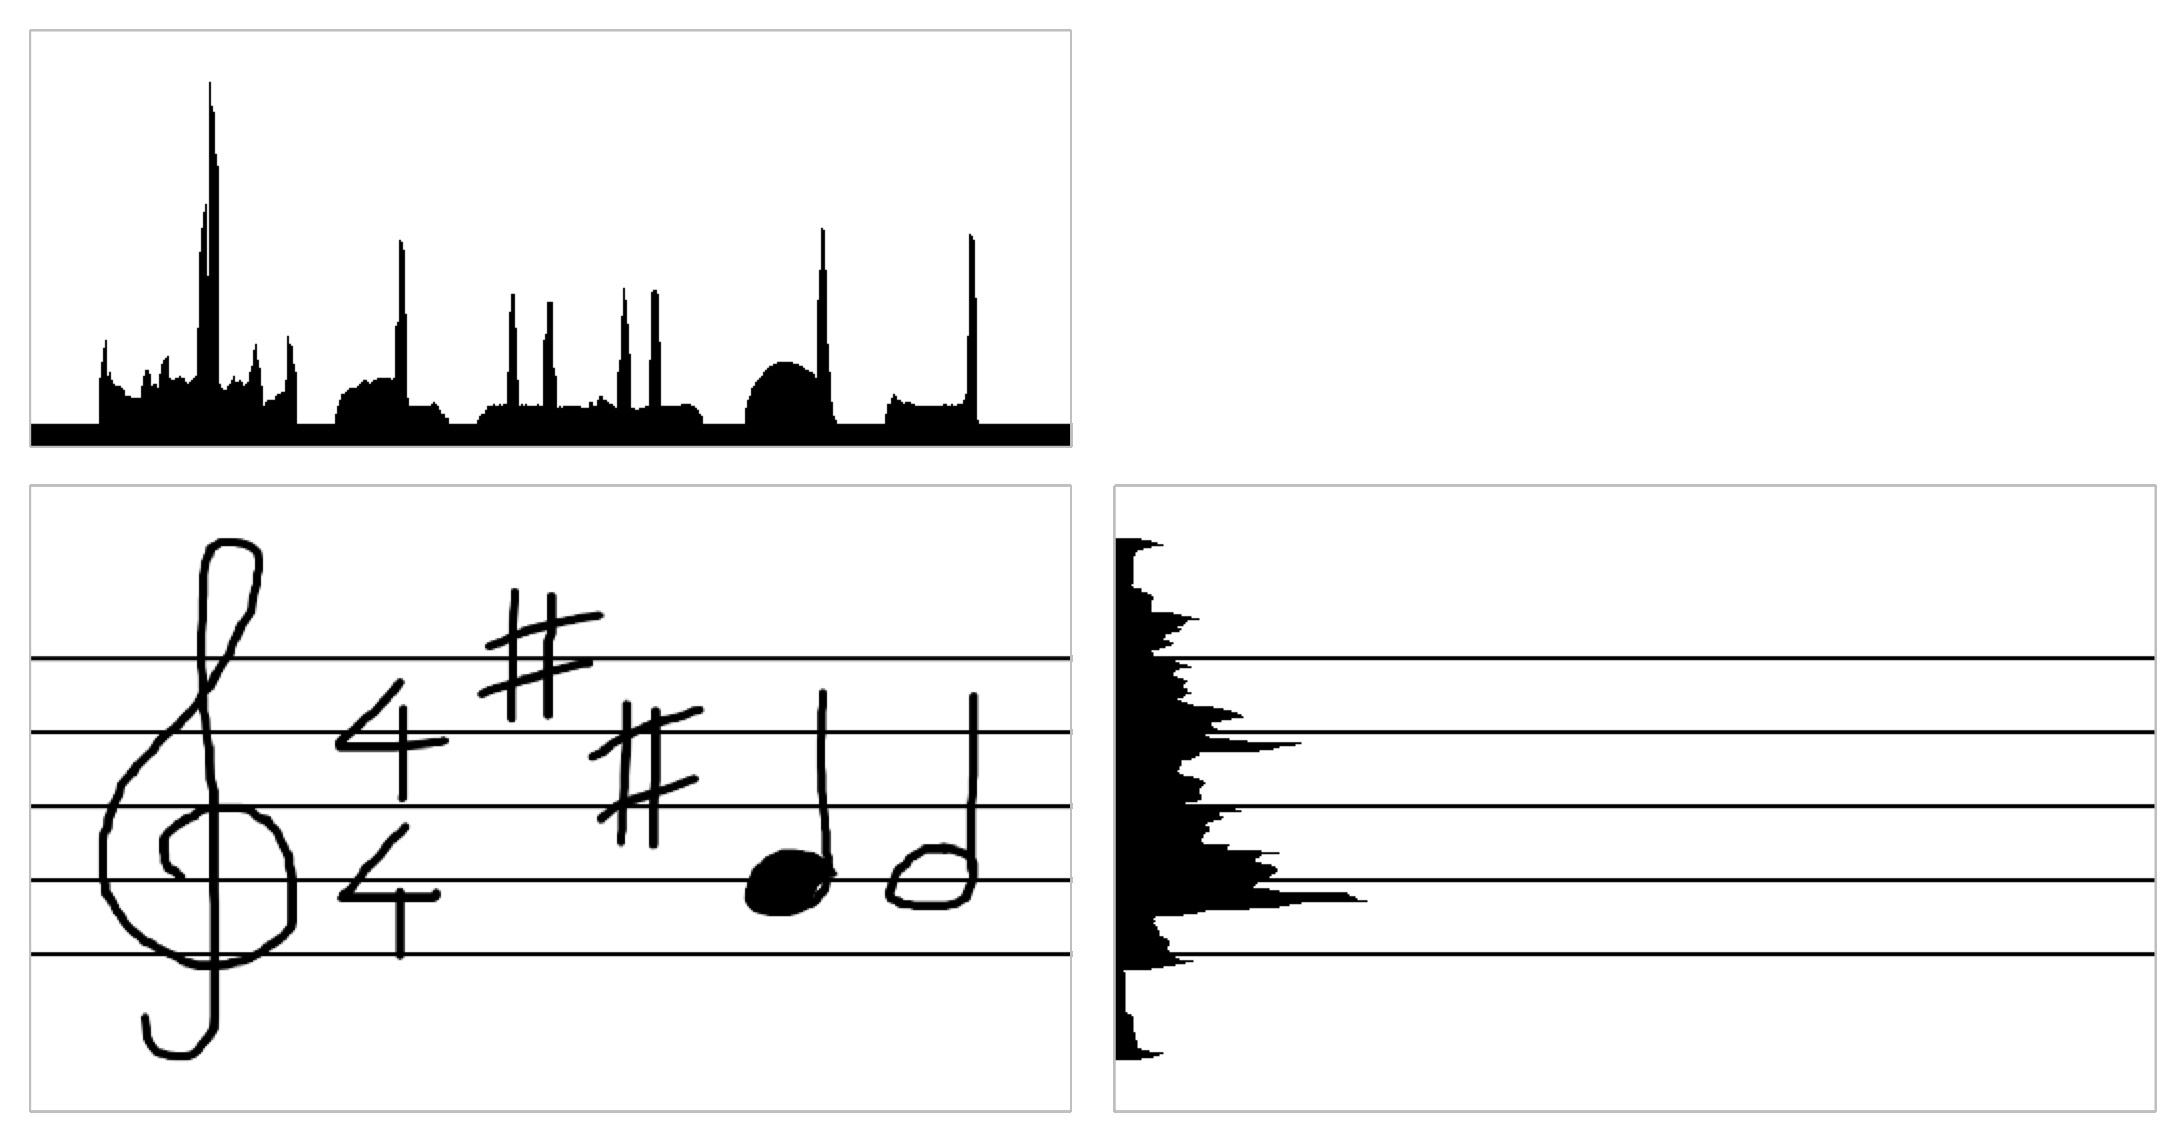
\includegraphics[width=\linewidth]{gfx/background-omr/projection.png}
  \caption{Horizontal and Vertical Projections of handwritten music excerpt}
  \label{fig:stave-projection}
\end{figure}

An example section of score is shown in figure \ref{fig:stave-projection} along with it's horizontal and vertical projections.

\subsection{Defects and Difficulties}

There are two regular types of error that can cause issues during segmentation, \textbf{touching objects} and \textbf{broken objects}. Since these are likely to occur a lot more regularly given the freedom allowed by handwritten music and the a beginner's learning curve, it is important that the application is able to spot (and subsequently feed back on) these errors.

\subsubsection{Touching Objects}

Touching objects are usually identifiable via a vertical projection profile \todo{reference projections} but can cause issues when segmenting components using \todo{Ref connected component} connected component analysis as it causes what were intended to be two separate objects to appear as one.

\todo[inline]{Examples of touching objects}

In a printed score, you can use \todo{ref template matching} template matching in order to separate the components but when they are handwritten, it's more likely I will have to rely on using projections to find the point of minimal intersection \todo{Reference to where I do split\_x and split\_y}

\subsection{Template Matching}

I've also attempted some examples of image segmentation using template matching, extracting components like the note head from the whole note as seen in Figure \ref{fig:templatematch}.

\begin{figure}[h!]
  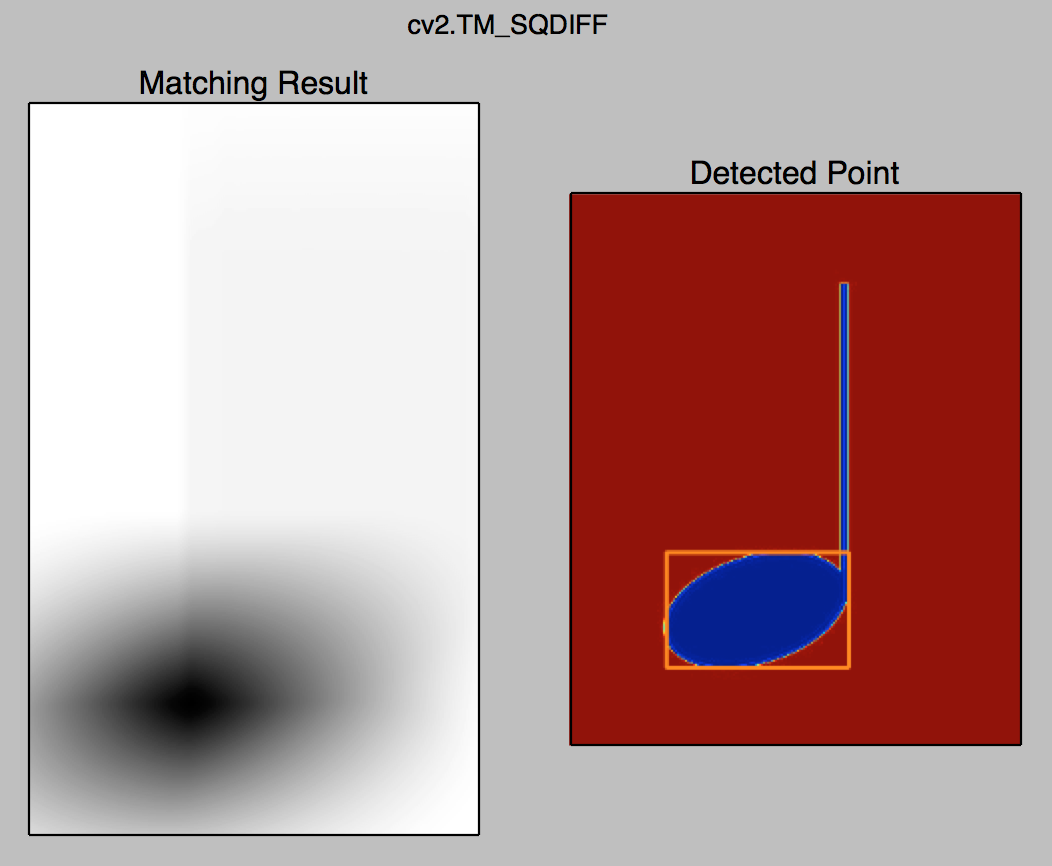
\includegraphics[width=0.6\linewidth]{gfx/template.png}
  \centering
  \caption{Example of extracting note heads using template matching}
  \label{fig:templatematch}
\end{figure}

In this example, I've used the OpenCV library and utilised the SQ\_DIFF method (or sum of squared differences), to find similar image regions which is a popular method of producing a `matching' score.

This involves analysing each pixel in an image (or a region of an image) and comparing it to a reference pixel in a template. The score for two $n \times m$ images $x$ and $y$ is therefore generated using:

$$SSD_{xy} = \sum_{i = 0}^m \sum_{j = 0}^n (x(i, j) - y(i, j))^2$$

In the example I gave previously, we're only looking for a subsection or a partial template. We therefore if image $x$ is $m \times n$ and image $y$ is $a \times b$in size where $m \le a \land n \le b$, we can search each possible position $(k, l)$ for $y$ in $x$ with:

$$SSD_{xy}(k, l) = \sum_{i = 0}^m \sum_{j = 0}^n (x(i + k, j + l) - y(i, j))^2$$

and whichever positioning gives us the highest score is likely to be the best match.




\section{Component Features}

\subsection{Basic Features}

Some basic features extracted from a component are:

\begin{enumerate}
  \item X Position
  \item Y Position
  \item Height
  \item Width
  \item 
\end{enumerate}

In some cases, x and y position on the staff are used in classification but for my purposed I have decided to perform classification assuming no prior knowledge. There might be exercises or free-drawing where a child doesn't want to have to follow the rules which apply to a normal score of music but rather draw specific components.

\subsection{Vertical and Horizontal Holes}

The average number of vertical and horizontal holes is used by \cite{fujinaga1996adaptive} and are topological properties in that they're generally scale invariant and as defined by \cite{burger2009principles} ``do not describe the shape of a region in continuous terms; instead, they capture its structural properties".

Average vertical and horizontal holes can be calculated by analysing the columns and rows respectively and counting the number of segments which do not have a solid pixel in (the runs of 0s). For example, for average horizontal holes we would count the number of white segments per row and total them up, averaging by the number of rows. Similarly with columns for vertical holes.

\subsection{Moments}

I use low level moments in this project to extract information like region area and centroid coordinates, however I wasn't able to get to grips with some of the higher order moments used by \cite{fujinaga1996adaptive,arabelo} to represent rotation, skew and other properties which may go some way to explaining my failed classifier in \cref{fig:knn-stats} (\cref{sec:knn-stats}) as my implementation may have simply been wrong. Since I achieved good classification results I was content to admit my shortcomings and stick to using a downsampled after that.

\subsubsection{Ordinary Definition}

As in \cite{burger2009principles} a moment of the order $p, q$ for an image or region $I(x,y)$ can be defined by \cref{eqn:general-moment}.

\begin{equation}\label{eqn:general-moment}
  m_{pq} = \sum_{x, y \in \mathbb{R}} I(x,y) \dot x^p y^q
\end{equation}

Since we're dealing with binary regions, we will only be considering the pixels of value 1, therefore since other pixels in $I(x,y)$ will be 0 we can simplify the general equation to \cref{eqn:general-moment-simple}.

\begin{equation}\label{eqn:general-moment-simple}
  m_{pq} = \sum_{x, y \in \mathbb{R}} x^p y^q
\end{equation}

\subsubsection{Zeroth Order Moments}

Zeroth order moments can be used to calculate the area of a binary region. The zero moment can be calculated using \cref{eqn:0-moment}

\begin{equation}\label{eqn:0-moment}
  m_{0} = \sum_{x, y \in \mathbb{R}} x^0 y^0 = \sum_{x, y \in \mathbb{R}} 1
\end{equation}

\subsubsection{First Order Moments}

The first order moments $m{01}$ and $m_{10}$ are use to obtain the centre of mass of a component at $(\bar{x}, \bar{y})$.

\begin{equation}\label{eqn:1-moment-mass}
\bar{x} = \frac{m_{10}}{m_{00}}, \bar{y} = \frac{m_{01}}{m_{00}}
\end{equation}

\subsection{Run Length Encoding}
\label{sec:tb-rle}

\acrfull{RLE} is something which is regularly mentioned in regard to OMR, it involves taking a pixel based image and converting what would be a huge amount of information into a more compact format by establishing ``runs'' of identical pixels which are in a contiguous block.

For a two dimensional binary image a run of pixels can be represented by it's row, column, value and run length \parencite[p. 27-28]{burger2009principles} as seen in \cref{table:rle-2d}

\begin{table}[H]

    \begin{tabularx}{\textwidth}{ X | X }
        \toprule
        Example & RLE $(\textbf{row}, \textbf{column}, \textbf{value}, \textbf{length})$\\
        \midrule

        $$\begin{bmatrix}
        1 & 2 & 2 & 3  \\
        3 & 3 & 3 & 1  \\
        1 & 1 & 5 & 5  \\
        5 & 5 & 2 & 2
        \end{bmatrix}$$

        &
        {[} (0, 0, 1, 1), (0, 1, 2, 2), (0, 3, 3, 1), \newline
        (1, 0, 3, 3), (1, 3, 1, 1), (2, 0, 1, 2), \newline
        (2, 2, 5, 2), (3, 0, 5, 2), (3, 2, 5, 2) {]} \\
        \ & \ \\
    \bottomrule
    \end{tabularx}

    \caption{2D Greyscale Image}
    \label{table:rle-2d}
\end{table}


\begin{table}[H]
    \begin{tabularx}{\textwidth}{ X | X }
        \toprule
        Example & RLE $(\textbf{value}, \textbf{length})$\\
        \midrule

        {[} 1, 2, 2, 3, 3, 3, 3, 1, 1, 1, 5, 5, 5, 5, 2, 2 {]}
        &
        {[} $(1, 1)$,
        $(2, 2)$,
        $(3, 4)$,
        $(1, 3)$,
        $(5, 4)$,
        $(2, 2)$ {]} \\
    \bottomrule
    \end{tabularx}

    \caption{1D Flattened Greyscale Image}
    \label{table:rle-1d}
\end{table}

\begin{table}[H]
    \begin{tabularx}{\textwidth}{ X | X }
        \toprule
        Example & RLE $\langle \textbf{value}, \textbf{length} \rangle$\\
        \midrule

        {[} 0, 0, 0, 1, 1, 1, 0, 0, 1, 1, 1, 1 {]}
        &
        {[} 0, 3, 3, 2, 4 {]} (first bit sets ordering)\newline
        {[} 3, 3, 2, 4 {]} (assuming initial bit is 0) \\
    \bottomrule
    \end{tabularx}

    \caption{1D Flattened Binary Image}
    \label{table:rle-1d-binary}
\end{table}

If you then reshape this 2D image into a one dimensional array (retrieving and reshaping it to it's 2D representation later), you can remove 50\% of the compressed data (row and column) as seen in \cref{table:rle-1d}

If we are using binary data we can simplify this further, simply tracking the initial bit, then recording runs of alternating values as seen in \cref{table-1d-binary}, we can simplify this further with the additional assumption \parencite{fujinaga1996adaptive} that the sequence will start with a 0, removing the need for the initial bit. If the sequence begins with a 1 we just start with an entry of length 0. Since a lot of musical entities don't touch the top left corner, this is the implementation I have used.

\section{Classification}

\subsection{Normalized Cross Correlation}

Normalized cross correlation enables (in the context of this application) a pixel-wise comparison of two images, resulting in a score between $[-1, 1]$ where 1 indicates a perfect match \eg the images are the same and $-1$ indicates the images are precisely the opposite of each other. The overall effect is to penalise the score for each pixel which is different in one image than the other. The normalisation is designed to help in images where the brightness and light levels vary but it works fine on binary images too.

An NCC score between two binary images $F$ and $G$ of the same dimension can be calculated by using \cref{eqn:ncc}.

\begin{lequation}\label{eqn:ncc}
  \frac{1}{N} \sum_{x,y} \frac{\left( f(x,y) - \bar{f}\right)\left( g(x,y) - \bar{g}\right)}{\sigma_{f} \sigma_{g}}
\end{lequation}

Where $N = w \times h$ (the number of pixels in the image), $f(x,y)$ and $g(x, y)$ represent the pixel in row y column x for the respective images, $\bar{f}, \bar{g}$ represent the average pixel values for each image and $\sigma_{f},  \sigma_{g}$ are the standard deviations of the two images. 

\subsection{Nearest Neighbour}

The \acrfull{KNN} algorithm is an example of instance based learning and works by extracting a set of features for each sample and using this `feature vector' to represent each sample in a multidimensional vector space.

Once this space has been generated, new samples may be classified by generating their feature vector and calculating the $k$ closest or `most similar' samples in the model by way of a distance calculation. By considering the $k$ closest samples, a consensus can be reached and the new sample is classified according to the label with the greatest majority in the $k$ nearest neighbours as seen in \cref{fig:knn-example}.

 \begin{figure}[h!]
   \centering
   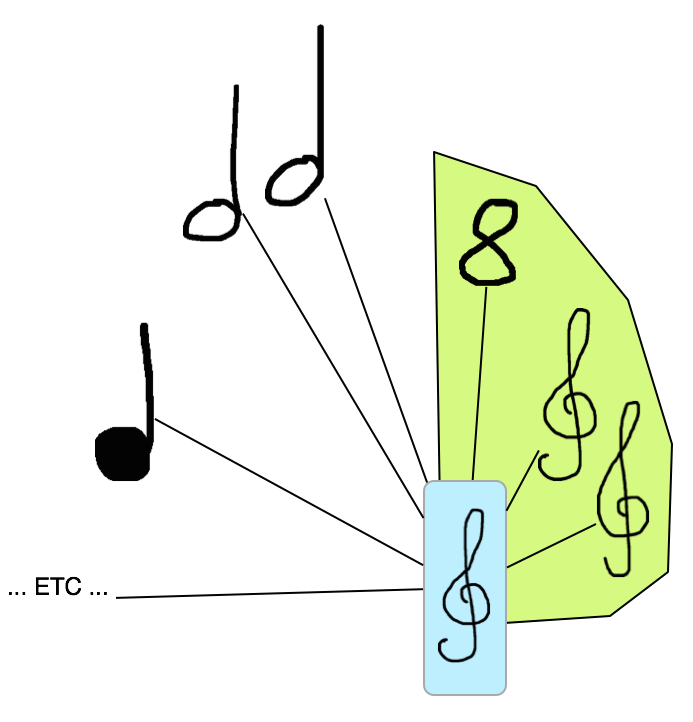
\includegraphics{gfx/techniques/knn-entities.png}
   \caption{KNN example using musical symbols and a K value of 3. The new symbol being classified is highlighted blue and the three closest three entities in green. In this case, the sample would be classified as a treble clef}
   \label{fig:knn-example}
 \end{figure}

The two most critical aspects of the KNN classifier are the distance method used and the number of neighbours considered. In order to maximise the accuracy of the classifier I perform several experiments to this effect in \cref{sec:implementation-classification}

\subsection{KNN Editing}

Although KNN can produce good results, the need to store all the data makes it less attractive. To reduce the data needed in classifiers you can use an edited KNN algorithm where the idea is to try and remove ``poor" samples which not only reduces the storage requirements but should also improve the accuracy of the classifier.

\subsubsection{Wilson Editing}
I originally came across the idea of edited KNN classifiers in \cite{fujinaga1996adaptive} in which he outlines the original KNN editing techniques from earlier work by \cite{wilson1972asymptotic}, (the algorithm for this editing technique is outlined in \cref{alg:knn-edit}). You can further extend the algorithm to multiple iterations (referred to by most as the multi-editing algorithm), repeating the process until no more poor samples are removed, at which point you save the model for use in classification, hopefully at a reduced dataset size.

\begin{algorithm}[H]
  \caption{KNN editing algorithm}
  \label{alg:knn-edit}

  \begin{algorithmic}
    \Procedure{EditModel}{model}
        \State trainingSamples = \Call{GetSamples}{model}
        \For {each sample in trainingSamples}
          \State classification = \Call{model.classify}{sample}
          \If{classification $\neq$ sample.classification}
            \Call{removeSample}{sample}
          \EndIf
    	\EndFor
    \EndProcedure
  \end{algorithmic}
\end{algorithm}

\subsubsection{Genetic Algorithms}

Although I actually decided not to employ the use of genetic algorithms in this project , they came up repeatedly in more recent research and so I felt it was worth a brief mention. Genetic algorithms for feature selection is nothing new, indeed it's used in \cite{fujinaga1996adaptive} for selecting which features to use in a classifier, a traditionally tricky problem when you have lots of features and need to work out which ones actually produce the best division of classes (though there are other techniques to do this too like PCA\footnote{Principal Component Analysis is used to find the dimension/variable in a feature vector which provides the highest variance possible. Features which provide small variance are of little help in a classification problem}), however in \ref{kuncheva1995editing} it is used specifically in editing a KNN classifier. The results suggested that it might perform comparably to wilson's technique and that it generally performed better than just using a random sample training set but that relative to multi-editing technique the authors state that they two could not be compared due to an inability to properly evaulate the power of the multi-edit algorithm.

It seems that right now, early investigations are being performed into whether genetic algorithms can be used to improve KNN classifiers but as of right now you can't say that they perform much better than existing techniques.
\section{Scoring \& Evaluation}

\subsection{NCC}

\todo[inline]{NCC: Upside: Easy to create a score from, set a threshold for 'good' then just divide and give stars}
\todo[inline]{NCC: Downside: Small images lead to big score differences for seemingly small image differences}
\todo[inline]{NCC: Downside: Wasn't ranking the images in the same order that a teacher would}
\todo[inline]{NCC: Downside: Doesn't tell a student what they did wrong, just a black box score, is that all that's needed? - NO}

\subsection{HOG}

\todo[inline]{Similar to NCC, slightly more accurate but more intensive to calculate, see Delteil}

\subsection{Image Difference}

If you're handling simple 1 bit images, you can perform a simple image difference which just takes the first image, XOR'd with the second. The result (shown in Figure \ref{fig:crotchet-diff}) is a simple highlighting of the difference between the two.

\begin{figure}[h!]
  \centering
  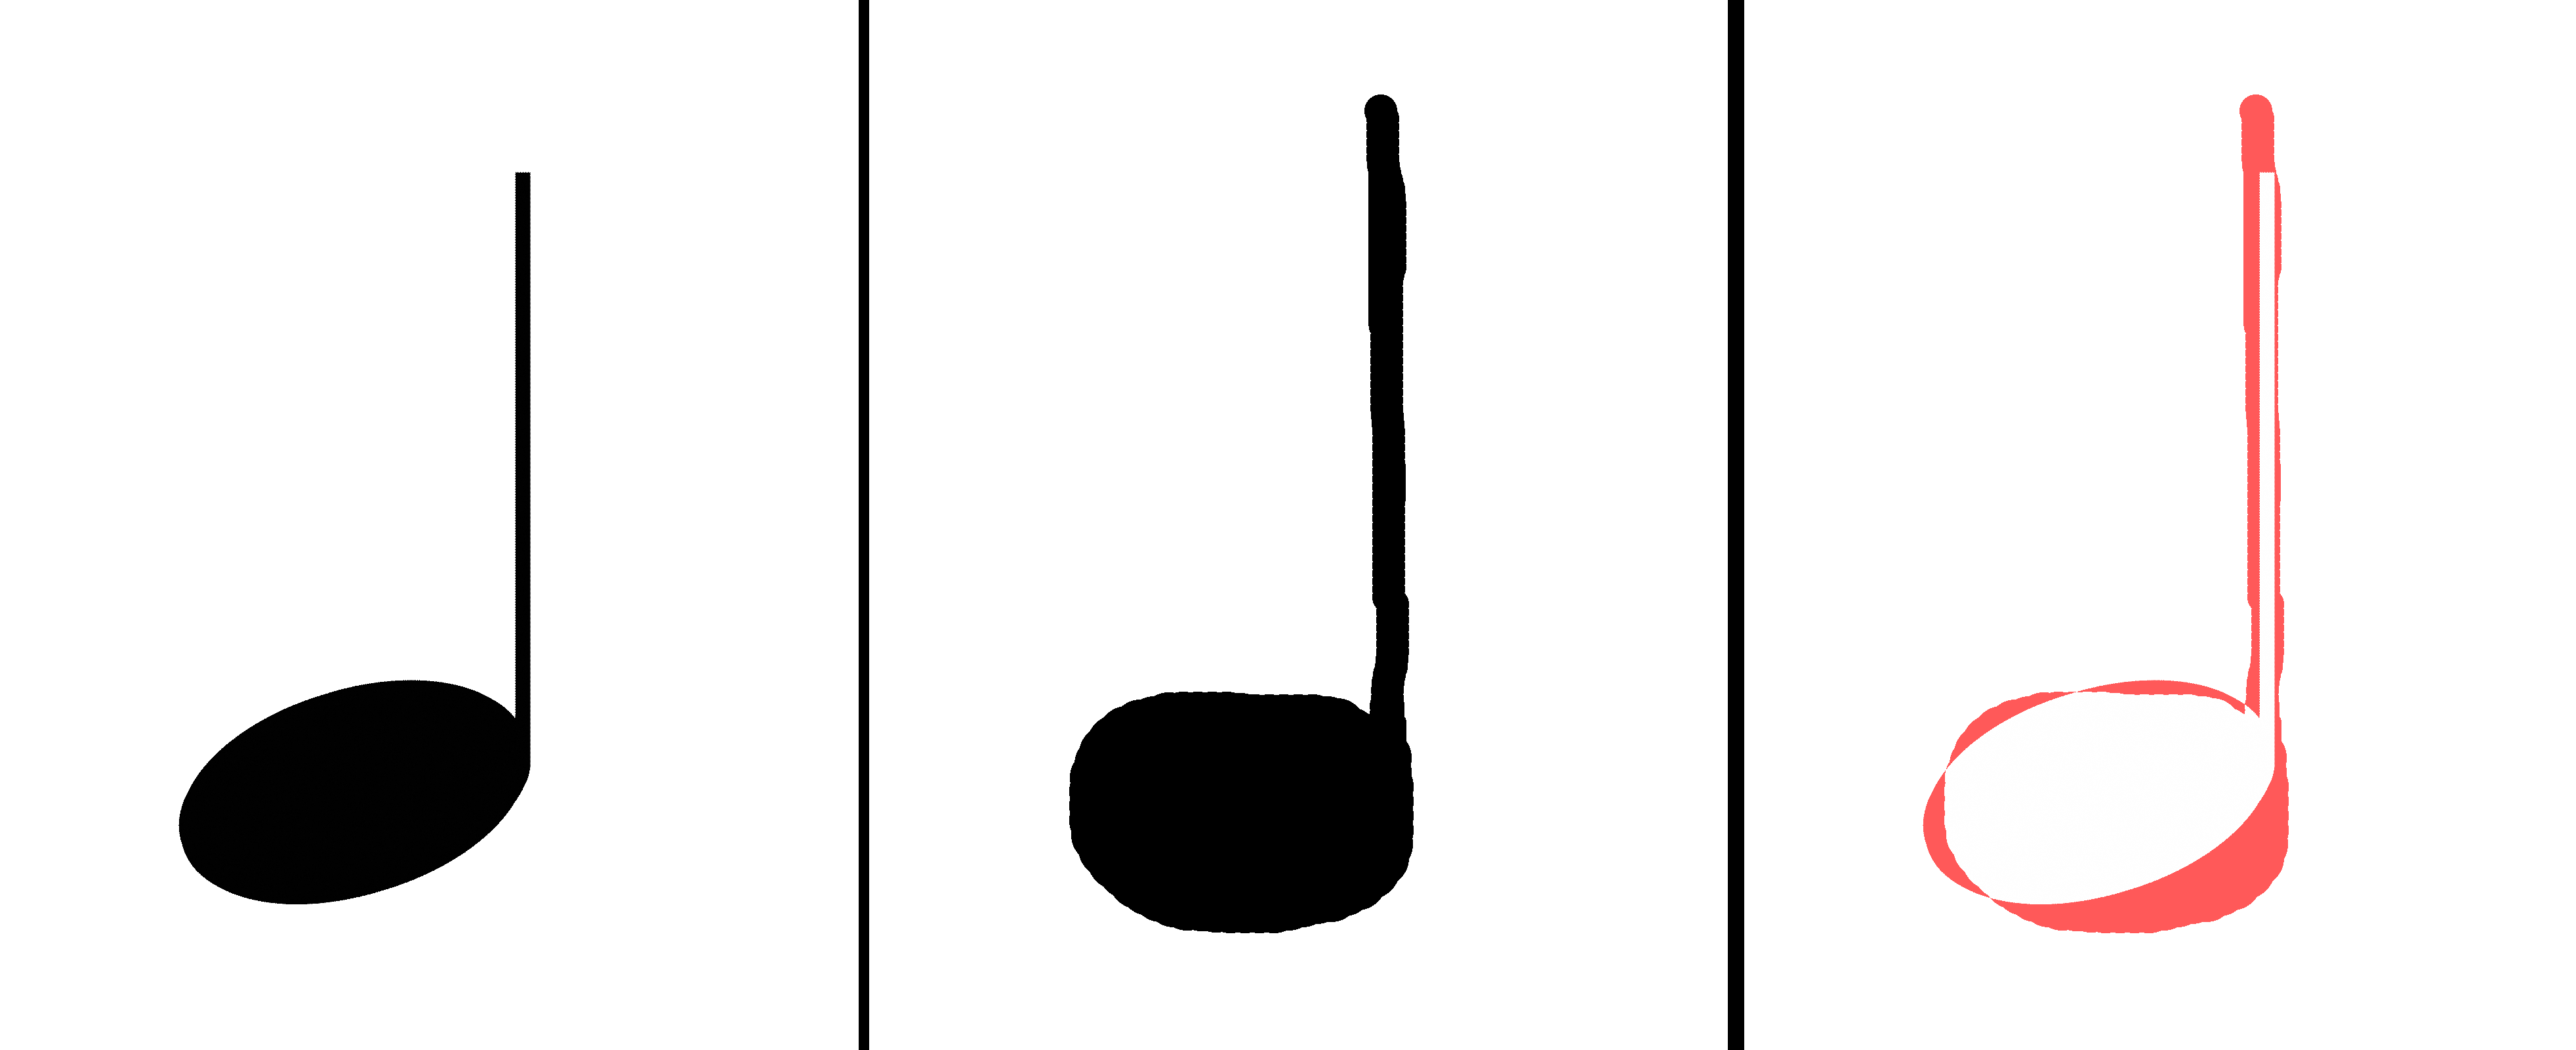
\includegraphics[width=\linewidth]{gfx/crochet-all.png}
  \caption{Highlighting differences between a perfect and a hand-drawn crochet}
  \label{crotchet-diff}
\end{figure}

\todo[inline]{Image Difference: Upside: Very visual, clear what's wrong}
\todo[inline]{Image Difference: Downside: Sensitive to the blob size, means stem errors are less likely to impact the score}

\subsection{Skeletonization}

\todo[inline,color=red]{Skeletonization - Write
\clearpage

\chapter{Techniques}

\section{Identification}\label{sec:identification}

As outlined in \cref{sec:techniques} above, a key challenge is identifying and isolating the various components which are going to be analysed. \cref{sec:segmentation} outlines from the research conducted and which methods were selected for segmentation, feature extraction and allocation of pitch, duration and other properties.

\subsection{Segmentation}\label{sec:segmentation}

In order to perform a decomposition of the manuscript, within \noteED I perform multiple stages of segmentation combined with classification. For the purposes of demonstration I will be following the identification process using the manuscript example in \cref{fig:canvas-initial}.

\begin{figure}[hbt]
  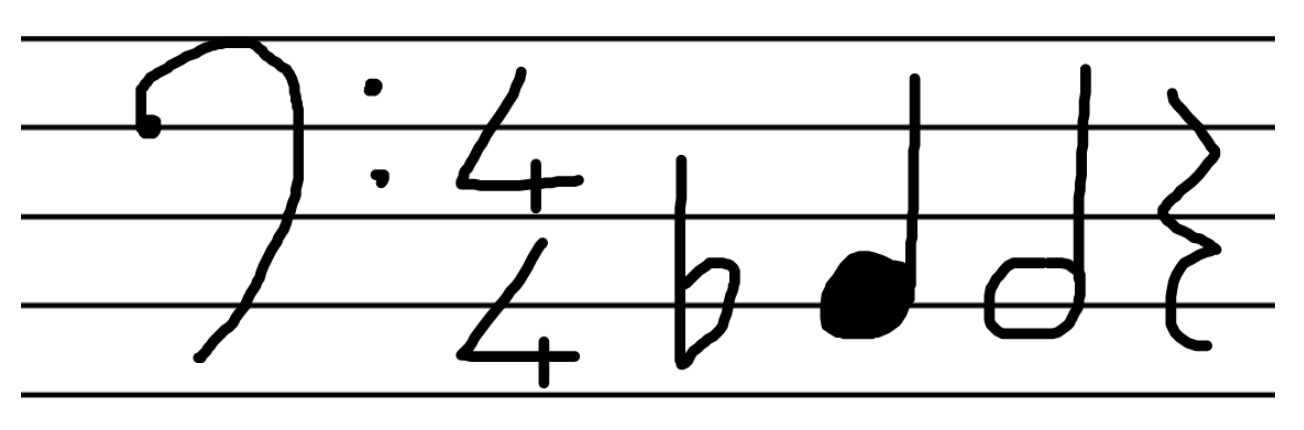
\includegraphics[width=\linewidth]{gfx/techniques/labelling/initial.png}
  \caption{The initial clean manuscript attempt}
  \label{fig:canvas-initial}
\end{figure}
\subsubsection{Initial Segmentation}

Connected component analysis (see \cref{sec:connected-component-analysis}) is performed to isolate the individual components on the stave, resulting in the first stage of component segmentation seen in \cref{fig:canvas-segmentation-1}.

\begin{figure}[hbt]
  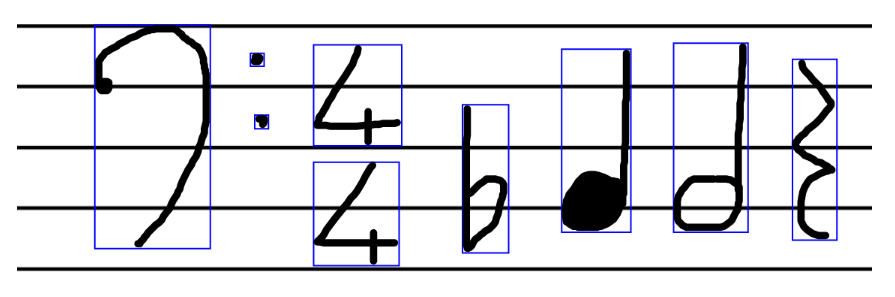
\includegraphics[width=\linewidth]{gfx/techniques/labelling/initial-segmentation.png}
  \caption{After initial segmentation of \cref{fig:canvas-initial}}
  \label{fig:canvas-segmentation-1}
\end{figure}

The components are then classified using the first of two KNN classifiers (KNN1 - discussed below in \cref{sec:implementation-classification}) which results in the basic labelling of the manuscript components seen in \cref{fig:canvas-classified-1}.

\begin{figure}[hbt]
  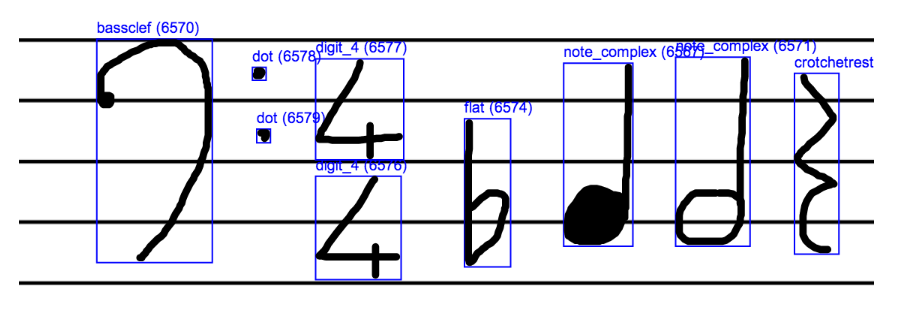
\includegraphics[width=\linewidth]{gfx/techniques/labelling/initial-classification.png}
  \caption{After first level classification of \cref{fig:canvas-segmentation-1}}
  \label{fig:canvas-classified-1}
\end{figure}

The \emph{note\_complex} and \emph{split\_x/split\_y} components are divided into sub-components using techniques such as stem removal (\cref{sec:stem-removal}) and vertical projections (\cref{sec:projections}) respectively. The new set of components are classified using one of the specialised classifiers, the original KNN1 classifier in the case of split components or the KNN2 classifier for note subcomponents to produce the more detailed component labelling in \cref{fig:canvas-segmentation-classification-2}.

\begin{figure}[hbt]
  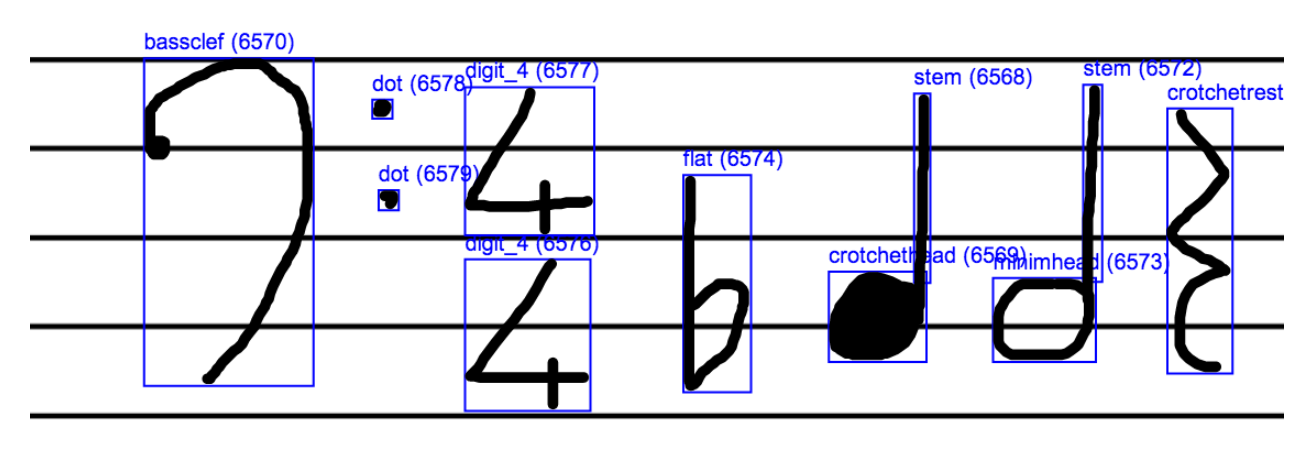
\includegraphics[width=\linewidth]{gfx/techniques/labelling/secondary-segmentation-classification.png}
  \caption{After second level segmentation and classification of \cref{fig:canvas-classified-1}. Note the stems are now labelled}
  \label{fig:canvas-segmentation-classification-2}
\end{figure}

No further segmentation is performed on the components after this point.

\subsubsection{Stem Removal}\label{sec:stem-removal}

In order to split up a \emph{note\_complex} into heads, tails, beam, stem etc, the first step is to try and isolate the stems. We can do this by removing horizontal runs of black pixels which are above a threshold greater than the typical width of a stem. Since runs like this appear at the intersection of the stem with other components, the result is a large number of new regions in the image, one of which is likely to be the stem.

To establish which region is a stem and remove any noise, we look for regions which are within a set aspect ratio (I use $1:2$, obtained experimentally and designed to catch angled stems as well as very vertical ones) and a height above a minimum threshold (I use $40$px, also obtained experimentally).

\begin{figure}[H]
  \centering

  \begin{subfigure}[b]{.2\linewidth}
      \centering
      
\includegraphics[width=\linewidth]{gfx/techniques/stem-detection-1.png}
      \caption{The original component}
      \label{fig:stem-segmentation-1}
  \end{subfigure}
  \begin{subfigure}[b]{.2\linewidth}
      \centering
      
\includegraphics[width=\linewidth]{gfx/techniques/stem-detection-2.png}
      \caption{The original component}
      \label{fig:stem-segmentation-2}
  \end{subfigure}
  \begin{subfigure}[b]{.2\linewidth}
      \centering
      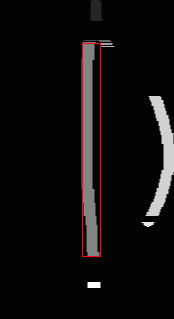
\includegraphics[width=\linewidth]{gfx/techniques/stem-detection-3.png}
      \caption{The original component}
      \label{fig:stem-segmentation-3}
  \end{subfigure}
  \begin{subfigure}[b]{.2\linewidth}
      \centering
      
\includegraphics[width=\linewidth]{gfx/techniques/stem-detection-4.png}
      \caption{The original component}
      \label{fig:stem-segmentation-4}
  \end{subfigure}

  \caption{The stages in stem detection for sharps}
  \label{fig:bar-line-types}
\end{figure}


\subsection{Feature Extraction}

\subsubsection{Resampling}

Using the pixels of an image as the features is an approach used in several of the papers I looked at \todo{Reference papers using images + resampling over features}, however in order to be able to compare feature vectors, they need to be the same size which means we need to resize the images to a common dimension.

To do this, I resize the images down using bilinear interpolation to an experimentally obtained dimension of $20\times50$px obtained in \cref{sec:knn}. The smaller dataset increases the speed at which a classifier can operate and I also found it to be comparable to if not more accurate than the feature vectors of larger images (\cref{table:knn-width-height-top}).

\subsubsection{Statistical Properties}
\label{sec:statistical-properties}

For my experimental statistical feature vector, I use techniques outlined in \cref{sec:component-features} to generate a feature vector comprising of the following properties:

\todo[inline,color=red]{Statistical Properties List which didn't bloody work}

\subsection{Classification}
\label{sec:implementation-classification}

Classifiers are created by taking a sets of previously labelled samples and building a model which provides the most accurate relation between the samples and their labels. This allows new samples to be classified using the model to apply the most likely (and hopefully, correct) label.

In order to maximise the accuracy of my classifications, I ran multiple experiments on different classifiers before deciding on which one I would apply in my application.

\subsubsection{K Nearest Neighbour}\label{sec:knn}

For the K Nearest Neighbour algorithm, I tried two different feature vectors, the first was using the statistical properties outlined in \cref{sec:statistical-properties} and the second was a resampled binary image flattened into a 1D array.

\paragraph{Statistical Feature Vector}
\label{sec:knn-stats}

An initial attempt at classification using statistical properties and a KNN classifier wasn't all that successful as you can see from the confusion matrix and accuracy scores in \cref{fig:knn-stats}. Most components were incorrectly classified as crotchet heads though I was unable to come up with a good explanation as to why and it's something which it would be interesting to investigate further in future.

\begin{table}
  \centering
  \begin{subtable}[b]{\linewidth}
    \tiny
    \begin{tabularx}{\textwidth}{r|XXXXXXXXXXXXXXXXXXXXXX}
         & \rot{crotchetrest}  & \rot{minimhead}  & \rot{note\_complex}  & \rot{bassclef}  & \rot{beam\_complex}  & \rot{sharp}  & \rot{semibreve}  & \rot{quaverrest}  & \rot{barline}  & \rot{quavertaildown}  & \rot{minimsemibreverest}  & \rot{flat}  & \rot{crotchethead}  & \rot{stem}  & \rot{trebleclef}  & \rot{digit\_8}  & \rot{natural}  & \rot{digit\_3}  & \rot{digit\_2}  & \rot{digit\_4}  & \rot{quavertailup}  & \rot{dot} \\
      \midrule
    crotchetrest & 0 & 0 & 0 & 0 & 0 & 0 & 0 & 0 & 0 & 0 & 0 & 0 & 44 & 0 & 0 & 0 & 0 & 0 & 0 & 0 & 0 & 0 \\
    minimhead & 0 & 16 & 0 & 0 & 0 & 0 & 0 & 0 & 0 & 0 & 0 & 0 & 48 & 0 & 0 & 0 & 0 & 0 & 0 & 0 & 0 & 0 \\
    note\_complex & 0 & 0 & 32 & 0 & 0 & 0 & 0 & 0 & 0 & 0 & 0 & 0 & 87 & 0 & 0 & 0 & 0 & 0 & 0 & 0 & 0 & 0 \\
    bassclef & 0 & 0 & 0 & 0 & 0 & 0 & 0 & 0 & 0 & 0 & 0 & 0 & 37 & 0 & 0 & 0 & 0 & 0 & 0 & 0 & 0 & 0 \\
    beam\_complex & 0 & 0 & 0 & 0 & 0 & 0 & 0 & 0 & 0 & 0 & 0 & 0 & 1 & 0 & 0 & 0 & 0 & 0 & 0 & 0 & 0 & 0 \\
    sharp & 0 & 0 & 0 & 0 & 0 & 6 & 0 & 0 & 0 & 0 & 0 & 0 & 46 & 0 & 0 & 0 & 0 & 0 & 0 & 0 & 0 & 0 \\
    semibreve & 0 & 0 & 0 & 0 & 0 & 0 & 1 & 0 & 0 & 0 & 0 & 0 & 37 & 0 & 0 & 0 & 0 & 0 & 0 & 0 & 0 & 0 \\
    quaverrest & 0 & 0 & 0 & 0 & 0 & 0 & 0 & 0 & 0 & 0 & 0 & 0 & 36 & 0 & 0 & 0 & 0 & 0 & 0 & 0 & 0 & 0 \\
    barline & 0 & 0 & 0 & 0 & 0 & 0 & 0 & 0 & 0 & 0 & 0 & 0 & 32 & 0 & 0 & 0 & 0 & 0 & 0 & 0 & 0 & 0 \\
    quavertaildown & 0 & 0 & 0 & 0 & 0 & 0 & 0 & 0 & 0 & 0 & 0 & 0 & 10 & 0 & 0 & 0 & 0 & 0 & 0 & 0 & 0 & 0 \\
    minimsemibreverest & 0 & 0 & 0 & 0 & 0 & 0 & 0 & 0 & 0 & 0 & 1 & 0 & 9 & 0 & 0 & 0 & 0 & 0 & 0 & 0 & 0 & 0 \\
    flat & 0 & 0 & 0 & 0 & 0 & 0 & 0 & 0 & 0 & 0 & 0 & 2 & 50 & 0 & 0 & 0 & 0 & 0 & 0 & 0 & 0 & 0 \\
    crotchethead & 0 & 0 & 0 & 0 & 0 & 0 & 0 & 0 & 0 & 0 & 0 & 0 & 133 & 0 & 0 & 0 & 0 & 0 & 0 & 0 & 0 & 0 \\
    stem & 0 & 0 & 0 & 0 & 0 & 0 & 0 & 0 & 0 & 0 & 0 & 0 & 60 & 24 & 0 & 0 & 0 & 0 & 0 & 0 & 0 & 0 \\
    trebleclef & 0 & 0 & 0 & 0 & 0 & 0 & 0 & 0 & 0 & 0 & 0 & 0 & 40 & 0 & 2 & 0 & 0 & 0 & 0 & 0 & 0 & 0 \\
    digit\_8 & 0 & 0 & 0 & 0 & 0 & 0 & 0 & 0 & 0 & 0 & 0 & 0 & 0 & 0 & 0 & 1 & 0 & 0 & 0 & 0 & 0 & 0 \\
    natural & 0 & 0 & 0 & 0 & 0 & 0 & 0 & 0 & 0 & 0 & 0 & 0 & 37 & 0 & 0 & 0 & 0 & 0 & 0 & 0 & 0 & 0 \\
    digit\_3 & 0 & 0 & 0 & 0 & 0 & 0 & 0 & 0 & 0 & 0 & 0 & 0 & 7 & 0 & 0 & 0 & 0 & 2 & 0 & 0 & 0 & 0 \\
    digit\_2 & 0 & 0 & 0 & 0 & 0 & 0 & 0 & 0 & 0 & 0 & 0 & 0 & 9 & 0 & 0 & 0 & 0 & 0 & 0 & 0 & 0 & 0 \\
    digit\_4 & 0 & 0 & 0 & 0 & 0 & 0 & 0 & 0 & 0 & 0 & 0 & 0 & 19 & 0 & 0 & 0 & 0 & 0 & 0 & 7 & 0 & 0 \\
    quavertailup & 0 & 0 & 0 & 0 & 0 & 0 & 0 & 0 & 0 & 0 & 0 & 0 & 11 & 0 & 0 & 0 & 0 & 0 & 0 & 0 & 3 & 0 \\
    dot & 0 & 0 & 0 & 0 & 0 & 0 & 0 & 0 & 0 & 0 & 0 & 0 & 27 & 0 & 0 & 0 & 0 & 0 & 0 & 0 & 0 & 15 \\
    \end{tabularx}
  \end{subtable}

  \vspace{0.8cm}

  \begin{subtable}[b]{.4\linewidth}
    \begin{tabularx}{\linewidth}{lll}
      \toprule
      Accuracy & Precision & Recall \\
      \midrule
      0.275 & 0.645 & 0.275 \\
      \bottomrule
    \end{tabularx}
  \end{subtable}

  \caption{KNN classifier results using statistical features}
  \label{fig:knn-stats}
\end{table}

\paragraph{Image Feature Vector}
\label{sec:knn-image}
For the resampled image features, I ran a series of trials for different dimensions from 10px to 100px in both width and height (in 10px increments), averaging 3 repeats per dimension (each with a different training/testing split) and then generating a matrix of accuracies (which can be seen in full in \cref{table:height-width-matrix}).

Since most objects on a stave have a more vertical aspect ratio, I first graphed the average and maximum of the scores for each different height across all widths to see if there were any trends such as taller images producing higher accuracy.

The results can be seen in \cref{fig:height-resample} and it seemed that in general, very short images ($\leq 20\text{px}$) gave worse results than tall ones but there wasn't anything conclusive and the gains from very tall images as opposed to fairly small images were minimal. Since there wasn't a height which clearly stood out, an analysis of the full matrix was done to find the highest scoring height and width combinations.

The top ten experimental accuracies from the tested dimensions are listed in \cref{table:knn-width-height-top} and I eventually selected $20\times50\text{px}$ as my resampled dimension, the reason being that although larger dimensions did technically produce better accuracies, they were only \emph{slightly} better and would have resulted in many more pixels in the feature vector, slowing down the process of building a classifier and testing samples.

\begin{figure}[H]
  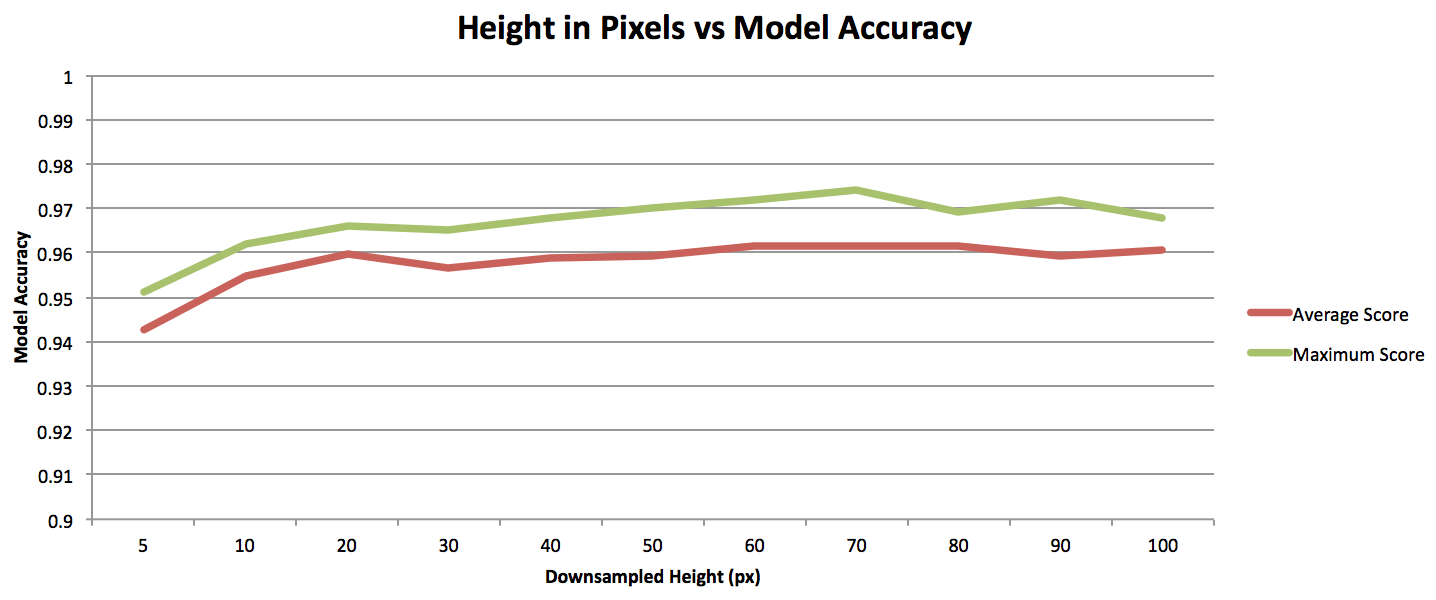
\includegraphics[width=\linewidth]{gfx/techniques/downsampling-height-vs-accuracy.png}
  \caption{The effect of resampled image height on accuracy}
  \label{fig:height-resample}
\end{figure}

\begin{table}[H]

    \begin{tabularx}{\textwidth}{ r X X X X }
    \toprule
    & Width & Height & Total Pixels & Accuracy \\
    \midrule
    & 50  & 70  & 3500 & 0.974 \\
    & 20  & 60  & 1200 & 0.971 \\
    & 20  & 70  & 1400 & 0.97 \\
    $\rightarrow$ & \textbf{20}  & \textbf{50}  & \textbf{1000} & \textbf{0.969} \\
    & 30  & 70  & 2100 & 0.969 \\
    & 100 & 70  & 7000 & 0.969 \\
    & 20  & 40  & 800  & 0.968 \\
    & 70  & 50  & 3500 & 0.967 \\
    & 60  & 60  & 3600 & 0.967 \\
    & 20  & 100 & 2000 & 0.967 \\
    \bottomrule
    \end{tabularx}

    \caption{Top 10 accuracy scores for different width and height combinations, the selection dimensions used in the classifier are highlighted and the full matrix can be found in \cref{table:height-width-matrix}}
    \label{table:knn-width-height-top}
\end{table}

\begin{table}[H]

    \begin{tabularx}{\textwidth}{ lXXXXXXXXXX }
    \toprule
    & \multicolumn{10}{c}{Width (px)} \\
    \cmidrule{2-11}
    Height (px) & 10   & 20   & 30   & 40   & 50   & 60   & 70   & 80   & 90   & 100  \\
    \midrule
    10          & 0.948 & 0.961 & 0.955 & 0.954 & 0.962 & 0.953 & 0.951 & 0.953 & 0.955 & 0.957 \\
    20          & 0.947 & 0.963 & 0.963 & 0.962 & 0.964 & 0.962 & 0.956 & 0.961 & 0.960 & 0.966 \\
    30          & 0.945 & 0.960 & 0.954 & 0.965 & 0.958 & 0.958 & 0.956 & 0.958 & 0.959 & 0.959 \\
    40          & 0.946 & 0.968 & 0.957 & 0.963 & 0.958 & 0.950 & 0.961 & 0.964 & 0.960 & 0.966 \\
    50          & 0.935 & 0.969 & 0.965 & 0.957 & 0.961 & 0.957 & 0.967 & 0.959 & 0.948 & 0.962 \\
    60          & 0.953 & 0.971 & 0.960 & 0.963 & 0.962 & 0.967 & 0.948 & 0.957 & 0.957 & 0.963 \\
    70          & 0.954 & 0.970 & 0.969 & 0.960 & 0.974 & 0.960 & 0.957 & 0.956 & 0.960 & 0.969 \\
    80          & 0.959 & 0.962 & 0.959 & 0.964 & 0.963 & 0.965 & 0.957 & 0.963 & 0.963 & 0.954 \\
    90          & 0.954 & 0.961 & 0.958 & 0.960 & 0.956 & 0.959 & 0.963 & 0.959 & 0.963 & 0.956 \\
    100         & 0.955 & 0.967 & 0.965 & 0.963 & 0.958 & 0.960 & 0.960 & 0.965 & 0.960 & 0.962 \\
    \bottomrule
    \end{tabularx}

    \caption{Accuracy Matrix for various Height and Width Downsampling Combinations}
    \label{table:height-width-matrix}
\end{table}

Initial results on attempting to distinguish between all components were positive and I was able to achieve around 93\% accuracy as seen in \cref{table:confusion-matrix-knn-img-all}.

\begin{figure}[H]
  \centering
  \begin{subtable}[b]{\linewidth}
    \small
    \begin{tabularx}{\textwidth}{r|XXXXXXXXXXXXXXXXXXXXX}
         & \rot{flat}  & \rot{trebleclef}  & \rot{crotchetrest}  & \rot{digit\_8}  & \rot{minimhead}  & \rot{crotchethead}  & \rot{digit\_2}  & \rot{digit\_4}  & \rot{quaverrest}  & \rot{semibreve}  & \rot{beam\_complex}  & \rot{quavertailup}  & \rot{bassclef}  & \rot{sharp}  & \rot{digit\_3}  & \rot{natural}  & \rot{barline}  & \rot{stem}  & \rot{quavertaildown}  & \rot{dot}  & \rot{minimsemibreverest} \\
      \midrule
    flat & 62 & 0 & 0 & 0 & 0 & 0 & 0 & 0 & 0 & 0 & 0 & 0 & 0 & 0 & 0 & 0 & 0 & 0 & 0 & 0 & 0 \\
    trebleclef & 0 & 53 & 0 & 0 & 0 & 0 & 0 & 0 & 0 & 0 & 0 & 0 & 0 & 0 & 0 & 0 & 0 & 0 & 0 & 0 & 0 \\
    crotchetrest & 0 & 0 & 37 & 0 & 0 & 0 & 0 & 0 & 0 & 0 & 0 & 0 & 0 & 0 & 0 & 0 & 0 & 0 & 0 & 0 & 0 \\
    digit\_8 & 0 & 0 & 0 & 0 & 0 & 0 & 0 & 0 & 0 & 0 & 0 & 0 & 0 & 0 & 0 & 0 & 0 & 0 & 0 & 0 & 0 \\
    minimhead & 0 & 0 & 0 & 0 & 43 & 0 & 0 & 0 & 0 & 3 & 0 & 0 & 0 & 0 & 0 & 0 & 0 & 0 & 0 & 0 & 0 \\
    crotchethead & 0 & 0 & 0 & 0 & 0 & 98 & 0 & 0 & 0 & 0 & 0 & 0 & 0 & 0 & 0 & 0 & 0 & 0 & 0 & 0 & 0 \\
    digit\_2 & 0 & 0 & 0 & 0 & 0 & 0 & 16 & 0 & 0 & 0 & 0 & 0 & 0 & 0 & 0 & 0 & 0 & 0 & 0 & 0 & 0 \\
    digit\_4 & 0 & 0 & 0 & 0 & 0 & 0 & 0 & 28 & 0 & 0 & 0 & 0 & 0 & 0 & 0 & 0 & 0 & 0 & 0 & 0 & 0 \\
    quaverrest & 0 & 0 & 0 & 0 & 0 & 0 & 0 & 0 & 35 & 0 & 0 & 0 & 0 & 0 & 0 & 0 & 0 & 0 & 0 & 0 & 0 \\
    semibreve & 0 & 0 & 0 & 0 & 0 & 0 & 0 & 0 & 0 & 37 & 0 & 0 & 0 & 0 & 0 & 0 & 0 & 0 & 0 & 0 & 0 \\
    beam\_complex & 0 & 1 & 0 & 0 & 0 & 0 & 0 & 0 & 0 & 0 & 0 & 0 & 0 & 0 & 0 & 0 & 0 & 0 & 0 & 0 & 0 \\
    quavertailup & 0 & 0 & 1 & 0 & 0 & 0 & 0 & 0 & 0 & 0 & 0 & 17 & 0 & 0 & 0 & 0 & 0 & 0 & 0 & 0 & 0 \\
    bassclef & 0 & 0 & 0 & 0 & 0 & 0 & 0 & 0 & 0 & 0 & 0 & 0 & 35 & 0 & 0 & 0 & 0 & 0 & 0 & 0 & 0 \\
    sharp & 0 & 0 & 0 & 0 & 0 & 0 & 0 & 0 & 0 & 0 & 0 & 0 & 0 & 55 & 0 & 0 & 0 & 0 & 0 & 0 & 0 \\
    digit\_3 & 0 & 0 & 0 & 0 & 0 & 0 & 0 & 0 & 0 & 0 & 0 & 0 & 0 & 0 & 5 & 0 & 0 & 0 & 0 & 0 & 0 \\
    natural & 0 & 0 & 0 & 0 & 0 & 0 & 0 & 0 & 0 & 0 & 0 & 0 & 0 & 0 & 0 & 49 & 0 & 0 & 0 & 0 & 0 \\
    barline & 1 & 0 & 0 & 0 & 0 & 0 & 0 & 0 & 0 & 0 & 0 & 0 & 0 & 0 & 0 & 0 & 20 & 18 & 0 & 0 & 0 \\
    stem & 0 & 5 & 0 & 0 & 0 & 0 & 0 & 0 & 0 & 0 & 0 & 0 & 0 & 0 & 0 & 0 & 3 & 92 & 0 & 0 & 0 \\
    quavertaildown & 0 & 0 & 0 & 0 & 0 & 0 & 0 & 0 & 0 & 0 & 0 & 0 & 0 & 0 & 0 & 0 & 0 & 0 & 9 & 0 & 0 \\
    dot & 0 & 0 & 0 & 0 & 0 & 7 & 0 & 0 & 0 & 0 & 0 & 0 & 0 & 0 & 0 & 0 & 0 & 2 & 0 & 38 & 0 \\
    minimsemibreverest & 0 & 0 & 0 & 0 & 0 & 0 & 0 & 0 & 0 & 0 & 0 & 0 & 0 & 0 & 0 & 0 & 0 & 6 & 0 & 5 & 0 \\
    \end{tabularx}
  \end{subtable}
  \vspace{0.8cm}
  \begin{subtable}[b]{.4\linewidth}
    \begin{tabularx}{\linewidth}{lll}
      \toprule
      Accuracy & Precision & Recall \\
      \midrule
      0.933 & 0.922 & 0.933 \\
      \bottomrule
    \end{tabularx}
  \end{subtable}
  \caption{Accuracy achieved using a KNN classifier trained on resampled 20x50px images}
  \label{table:confusion-matrix-knn-img-all}
\end{figure}

We can see that a few components in \cref{table:confusion-matrix-knn-img-all} are confused more than others, for example \emph{stems} and \emph{barlines}. To mitigate this, we can employ the use of hierarchical classification. Instead of trying to classify every single component at once, we can instead perform an initial `high level' classification, followed by further secondary classifications. The best example of this is a note. Instead of trying to separate a note straight away into heads stems and beams, it's sufficient to simply classify it as a `note\_complex' entity and perform more detailed classification of components later.

Using a two-stage classifier much more satisfactory results were achieved, with an initial classification accuracy of 98.5\% (\cref{fig:knn-level1}) and a secondary classification accuracy of 100\% (\cref{fig:knn-level2})!

\begin{figure}[H]
  \centering

  \vspace{0.4cm}

  \begin{subtable}[b]{\linewidth}
    \centering
    \small
    \begin{tabularx}{.8\textwidth}{r|XXXXXXXXXXXXXXXXX}
         & \rot{flat}  & \rot{digit\_4}  & \rot{trebleclef}  & \rot{crotchetrest}  & \rot{digit\_8}  & \rot{dot}  & \rot{digit\_3}  & \rot{digit\_2}  & \rot{semibreve}  & \rot{quaverrest}  & \rot{note\_complex}  & \rot{natural}  & \rot{bassclef}  & \rot{beam\_complex}  & \rot{sharp}  & \rot{barline}  & \rot{minimsemibreverest} \\
      \midrule
    flat & 55 & 0 & 0 & 0 & 0 & 0 & 0 & 0 & 0 & 0 & 0 & 0 & 0 & 0 & 0 & 0 & 0 \\
    digit\_4 & 0 & 24 & 0 & 0 & 0 & 0 & 0 & 0 & 0 & 0 & 0 & 0 & 0 & 0 & 0 & 0 & 0 \\
    trebleclef & 0 & 0 & 49 & 0 & 0 & 0 & 0 & 0 & 0 & 0 & 0 & 0 & 0 & 0 & 0 & 0 & 0 \\
    crotchetrest & 0 & 0 & 0 & 35 & 0 & 0 & 0 & 0 & 0 & 0 & 0 & 0 & 0 & 0 & 0 & 0 & 0 \\
    digit\_8 & 0 & 0 & 0 & 0 & 0 & 0 & 0 & 0 & 0 & 0 & 0 & 0 & 0 & 0 & 0 & 0 & 0 \\
    dot & 0 & 0 & 0 & 0 & 0 & 45 & 0 & 0 & 0 & 0 & 0 & 0 & 0 & 0 & 0 & 0 & 0 \\
    digit\_3 & 0 & 0 & 0 & 2 & 0 & 0 & 3 & 0 & 0 & 0 & 0 & 0 & 0 & 0 & 0 & 0 & 0 \\
    digit\_2 & 0 & 0 & 0 & 0 & 0 & 0 & 0 & 16 & 0 & 0 & 0 & 0 & 0 & 0 & 0 & 0 & 0 \\
    semibreve & 0 & 0 & 0 & 0 & 0 & 0 & 0 & 0 & 47 & 0 & 0 & 0 & 0 & 0 & 0 & 0 & 0 \\
    quaverrest & 0 & 0 & 0 & 0 & 0 & 0 & 0 & 0 & 0 & 35 & 0 & 0 & 0 & 0 & 0 & 0 & 0 \\
    note\_complex & 0 & 0 & 0 & 0 & 0 & 0 & 0 & 0 & 0 & 0 & 125 & 0 & 2 & 0 & 0 & 0 & 0 \\
    natural & 0 & 0 & 0 & 0 & 0 & 0 & 0 & 0 & 0 & 0 & 0 & 35 & 0 & 0 & 0 & 0 & 0 \\
    bassclef & 0 & 0 & 0 & 0 & 0 & 0 & 0 & 0 & 0 & 0 & 0 & 0 & 34 & 0 & 0 & 0 & 0 \\
    beam\_complex & 0 & 0 & 0 & 0 & 0 & 0 & 0 & 0 & 0 & 0 & 0 & 0 & 0 & 0 & 0 & 0 & 0 \\
    sharp & 0 & 2 & 0 & 0 & 0 & 0 & 0 & 0 & 0 & 0 & 0 & 0 & 0 & 0 & 60 & 0 & 0 \\
    barline & 0 & 0 & 0 & 0 & 0 & 0 & 0 & 0 & 0 & 0 & 0 & 0 & 0 & 0 & 0 & 27 & 0 \\
    minimsemibreverest & 0 & 0 & 0 & 0 & 0 & 3 & 0 & 0 & 0 & 0 & 0 & 0 & 0 & 0 & 0 & 0 & 3 \\
    \end{tabularx}
  \end{subtable}

  \vspace{0.8cm}

  \begin{subtable}[b]{.4\linewidth}
    \begin{tabularx}{\linewidth}{lll}
      \toprule
      Accuracy & Precision & Recall \\
      \midrule
      0.985 & 0.986 & 0.985 \\
      \bottomrule
    \end{tabularx}
  \end{subtable}

  \vspace{0.4cm}

  \caption{1st level KNN Classifier Results}
  \label{fig:knn-level1}
\end{figure}

\begin{figure}[H]
  \centering

  \vspace{0.4cm}

  \begin{subtable}[b]{.4\linewidth}
    \begin{tabularx}{\textwidth}{r|XXXXX}
         & \rot{minimhead}  & \rot{crotchethead}  & \rot{quavertailup}  & \rot{quavertaildown}  & \rot{stem} \\
      \midrule
    minimhead & 51 & 0 & 0 & 0 & 0 \\
    crotchethead & 0 & 118 & 0 & 0 & 0 \\
    quavertailup & 0 & 0 & 23 & 0 & 0 \\
    quavertaildown & 0 & 0 & 0 & 5 & 0 \\
    stem & 0 & 0 & 0 & 0 & 93 \\
    \end{tabularx}
  \end{subtable}

  \vspace{0.8cm}

  \begin{subtable}[b]{.4\linewidth}
    \begin{tabularx}{\linewidth}{lll}
      \toprule
      Accuracy & Precision & Recall \\
      \midrule
      1.0 & 1.0 & 1.0 \\
      \bottomrule
    \end{tabularx}
  \end{subtable}

  \vspace{0.4cm}

  \caption{2nd level KNN Classifier Results}
  \label{fig:knn-level2}
\end{figure}


\subsubsection{Neural Net}

Although neural networks are also common in OMR, I was unfortunately unable to extract any great results from them during my experiments. The best classification result I got was by using Hierarchical Classification, where the network achieved an accuracy of 80.38\% for the 1st level classifier as seen in \cref{fig:nn-classification-data}. I used trained the network using Backwards Propogation and used two hidden sigmoidal layers of 25 nodes each.
As more potential classes were added, unfortunately the accuracy just decreased and so I chose to use KNN as my classification technique.

It should be noted that further depth of research in this area fell outside the scope of this project and is not an area in which I have specific expertise. Many people have great success using neural networks for this and similar applications, achieving high accuracy rates and it's certainly something which is maybe worth coming back to again in future.

\begin{figure}[H]
  \centering

  \vspace{0.4cm}

  \begin{subtable}[b]{   \linewidth}
    \small
    \begin{tabularx}{\textwidth}{r|XXXXXXXXXXXXXXX}
    & \rot{crotchetrest} & \rot{semibreve} & \rot{dot} & \rot{flat} & \rot{digit\_2} & \rot{barline} & \rot{trebleclef} & \rot{sharp} & \rot{quaverrest} & \rot{digit\_3} & \rot{note\_complex} & \rot{natural} & \rot{digit\_4} & \rot{bassclef} & \rot{minimsemibreverest} \\
    \midrule
    crotchetrest       & 29 &  0 &  1 &  0  & 1 &  0 &  3 &  3 &  0 &  0 &   5  &  1  &  1  &  1  &  0 \\
    semibreve          &  0 & 45 &  0 &  0  & 0 &  0 &  0 &  0 &  0 &  0 &   1  &  0  &  0  &  0  &  0 \\
    dot                &  0 &  1 & 43 &  0  & 0 &  0 &  0 &  0 &  0 &  0 &   0  &  1  &  0  &  1  &  0 \\
    flat               &  0 &  0 &  0 & 43  & 0 &  0 &  0 &  3 &  0 &  0 &   8  &  1  &  1  &  0  &  0 \\
    digit\_2            &  0 &  0 &  1 &  0  & 5 &  0 &  0 &  0 &  0 &  0 &   4  &  0  &  0  &  0  &  0 \\
    barline            &  0 &  0 & 10 &  0  & 0 & 28 &  2 &  1 &  0 &  0 &   0  &  0  &  2  &  0  &  0 \\
    trebleclef         &  1 &  0 &  0 &  1  & 0 &  2 & 29 &  3 &  0 &  0 &   0  &  0  &  1  &  0  &  0 \\
    sharp              &  1 &  0 &  2 &  0  & 0 &  1 &  1 & 46 &  0 &  0 &   0  &  0  &  1  &  0  &  0 \\
    quaverrest         &  0 &  0 &  0 &  0  & 0 &  0 &  0 &  0 & 32 &  1 &   1  &  1  &  0  &  0  &  0 \\
    digit\_3            &  0 &  0 &  0 &  0  & 0 &  0 &  2 &  1 &  0 &  0 &   3  &  0  &  0  &  0  &  0 \\
    note\_complex       &  0 &  0 &  0 &  0  & 1 &  0 &  1 &  0 &  3 &  0 & 102  &  1  &  0  &  0  &  0 \\
    natural            &  0 &  0 &  0 &  0  & 0 &  0 &  2 &  1 &  0 &  0 &   1  & 31  &  0  &  0  &  0 \\
    digit\_4            &  1 &  1 &  0 &  0  & 0 &  2 &  3 &  4 &  0 &  0 &   4  &  0  & 10  &  0  &  0 \\
    bassclef           &  0 &  0 &  0 &  0  & 0 &  0 &  0 &  0 &  1 &  0 &   4  &  0  &  0  & 28  &  0 \\
    minimsemibreverest &  0 &  0 &  9 &  0  & 0 &  0 &  0 &  0 &  0 &  0 &   0  &  0  &  0  &  0  &  0 \\
    \end{tabularx}
  \end{subtable}

  \vspace{0.8cm}

  \begin{subtable}[b]{.4\linewidth}
    \begin{tabularx}{\linewidth}{lll}
      \toprule
      Accuracy & Precision & Recall \\
      \midrule
      0.804 & 0.797 & 0.804 \\
      \bottomrule
    \end{tabularx}
  \end{subtable}

  \vspace{0.4cm}

  \caption{1st level Neural Network Classifier Results}
  \label{fig:nn-classification-data}
\end{figure}

\subsection{Pitch}
\label{sec:pitch-identification}

For note heads and accidentals, it's important to know exactly where the centre of the note lies in order to correctly identify it's position on the stave. Doing this roughly is usually sufficient for OMR, however, since we would like to be able to feed back to the student if they aren't putting their notes in the right place or they're too big/small we need to be as accurate as possible.

Once the position has been determined, we can calculate the difference between that and the y coordinate of the various pitched components on the stave. Assigning the pitch which is closest using \cref{alg:note-assignment} results in a pitch assignment for pitched components, an example of which can be seen in \cref{fig:canvas-pitched}.

\begin{algorithm}[H]
\caption{Assigning a pitch to a component}
\label{alg:note-assignment}
\begin{algorithmic}[1]
\Procedure{GetNoteForComponent}{$component$}
    \State sum = \Call{GetComponentCentre}{$component$}
    \State min\_distance = $\infty$
    \State assigned\_pitch = None
    \For {each pitch in pitches}
      \State dist = \Call{ABS}{pitch\_coord - y}
      \If{dist $<$ min\_dist}
        \State min\_dist = dist
        \State allocated\_pitch = pitch
      \EndIf
	\EndFor
	\Return assigned\_pitch
\EndProcedure
\end{algorithmic}
\end{algorithm}

An example of a manuscript where the pitches have been established can be seen in \cref{fig:canvas-pitches}

\begin{figure}[hbt]
  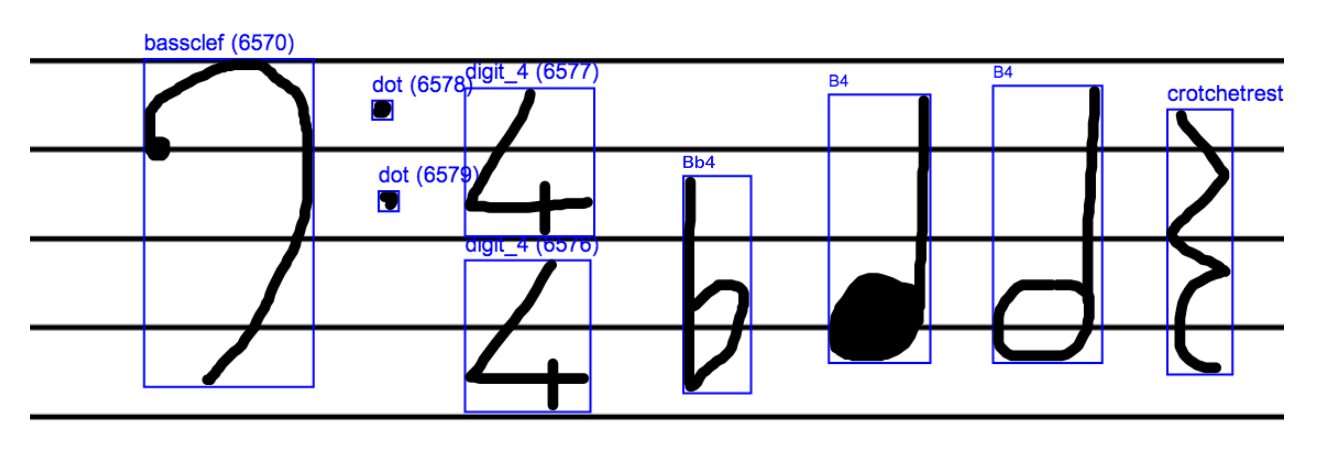
\includegraphics[width=\linewidth]{gfx/techniques/labelling/pitch.png}
  \caption{The manuscript after pitch analysis}
  \label{fig:canvas-pitches}
\end{figure}

For a rough estimate of note head position, the simplest method is to use a known position along the vertical axis, then use that as an estimate for the centre, indeed that's often what is done in standard OMR. However we can get a more accurate position using alternative techniques.

\subsubsection{Sharp Centres}
For the sharp centre, the centroid proved less than satisfactory as it was easily affected by the length of the lines (see the blue centres in \cref{fig:sharp-centroids}), whereas in reality the `centre' of a sharp is determined by the position of its island region in the middle.

By inverting the image and performing connected component segmentation, we can isolate the island region and after extracting the centroids from this region, we get a much more satisfactory identification of the sharp's centre, show in \cref{fig:sharp-centroids} by the intersecting red lines.

\begin{figure}[h!]
    \centering
    \begin{subfigure}[b]{.3\linewidth}
        \centering
        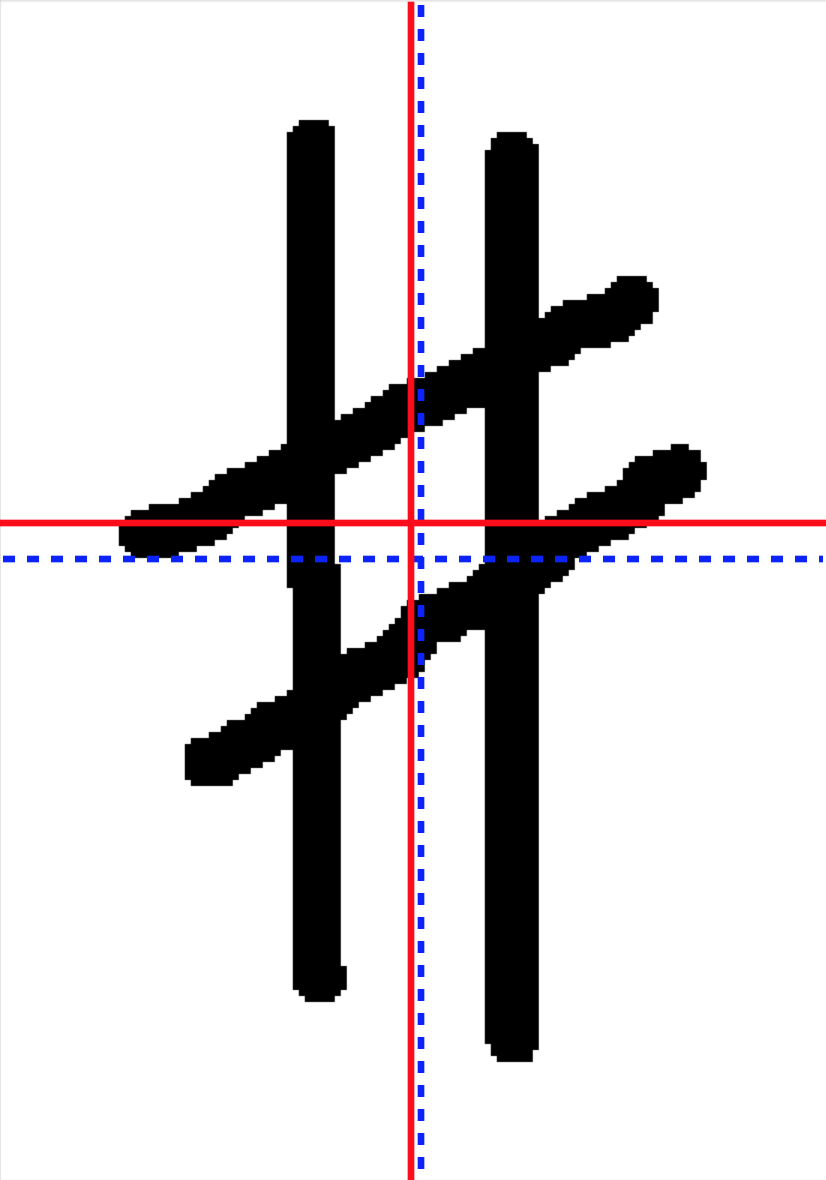
\includegraphics[height=5cm]{gfx/techniques/sharp-centroid-6109.png}
        \phantomsubcaption
    \end{subfigure}
    \begin{subfigure}[b]{.3\linewidth}
        \centering
        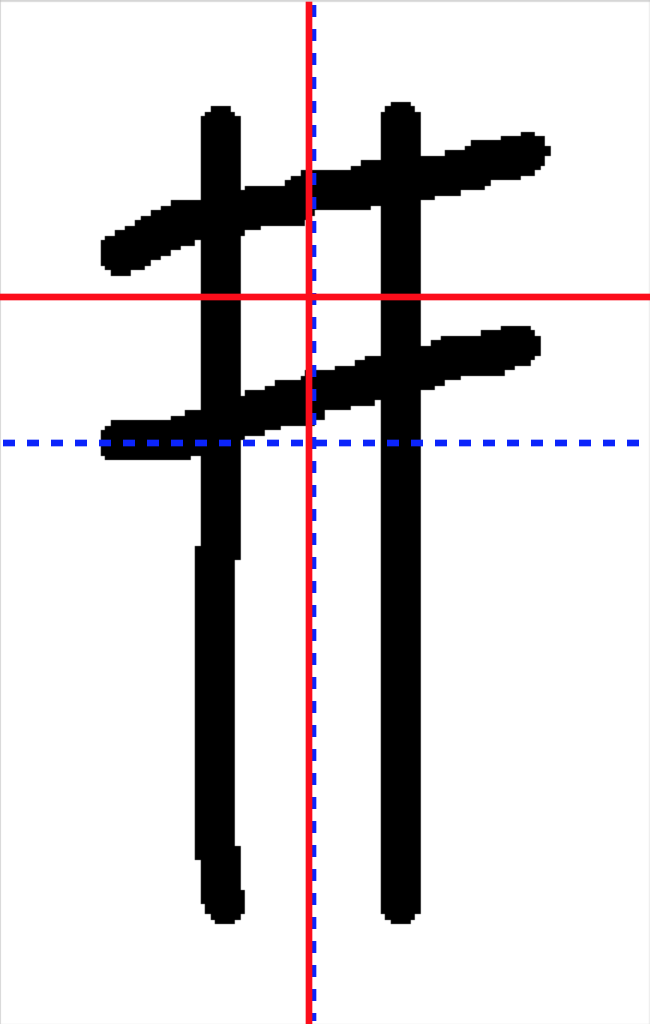
\includegraphics[height=5cm]{gfx/techniques/sharp-centroid-6110.png}
        \phantomsubcaption
    \end{subfigure}
    \begin{subfigure}[b]{.3\linewidth}
        \centering
        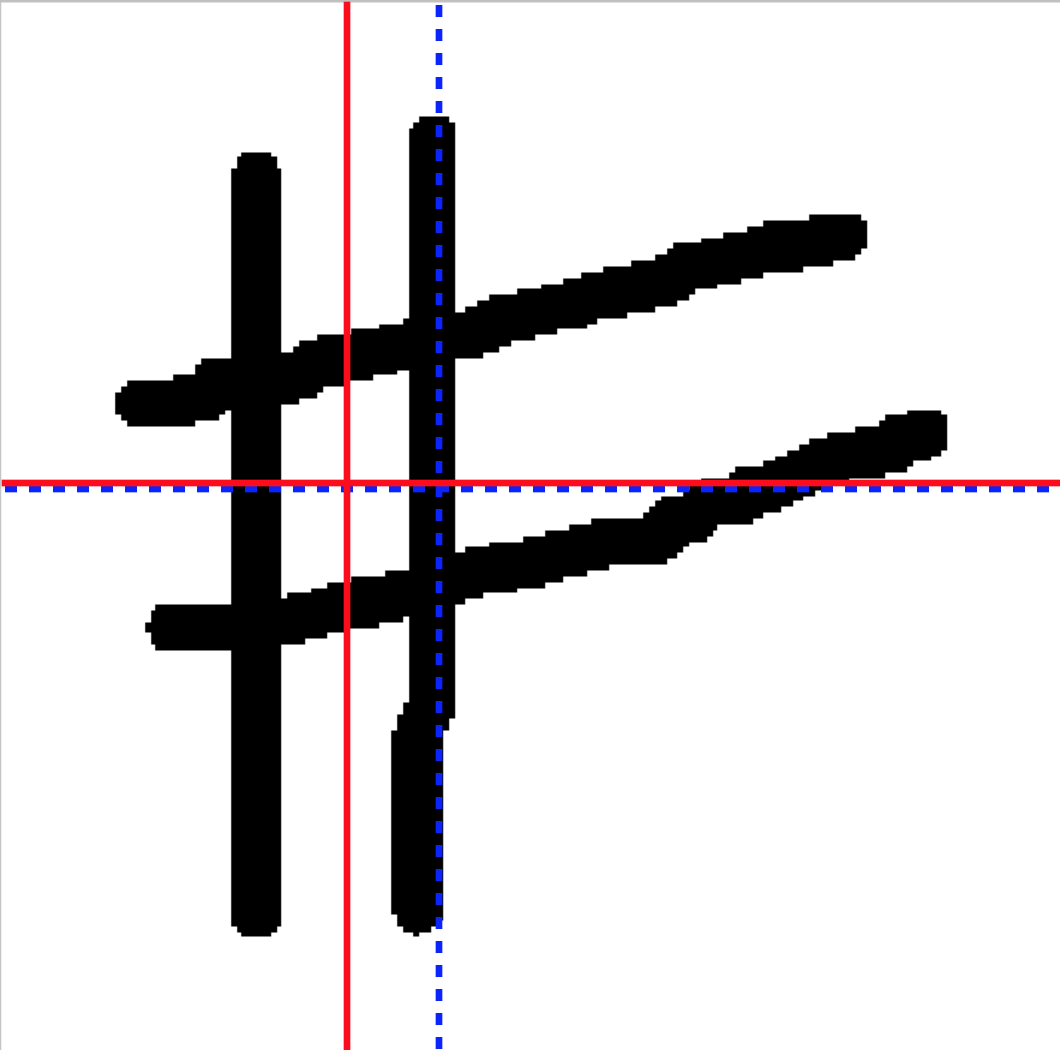
\includegraphics[height=5cm]{gfx/techniques/sharp-centroid-6108.png}
        \phantomsubcaption
    \end{subfigure}

  \caption{Identifying the true centres of the drawn sharps. Red intersecting lines show the true centres and blue intersecting lines show the centroid centres}
  \label{fig:sharp-centroids}
\end{figure}

\subsubsection{Flat Centres}

An unfortunate occurrence in flats during preliminary user testing was that of not joining the head up properly, an example of which can be seen in \cref{fig:flat-broken}. Ideally we would like to perform a similar technique to sharps, however we need some reliable way to compensate for potential breaks.

The first experiment I ran was to perform watershed segmentation by computing a distance transform on the flat, then by using the local maximum peaks as a starting point watershed segmentation was performed, resulting in the initial segmentation seen in \cref{fig:flat-broken-watershed}. From there, by merging neighbouring regions from smallest to largest, we can identify the `island' component (\cref{fig:flat-broken-merged}) and take the y coordinate of the centroid of this region.

\begin{figure}[H]
    \centering
    \begin{subfigure}[b]{.19\linewidth}
        \centering
        
\includegraphics[height=5cm]{gfx/techniques/scoring/flats/6193-original.png}
        \caption{Original}
        \label{fig:flat-broken}
    \end{subfigure}
    \begin{subfigure}[b]{.19\linewidth}
        \centering
        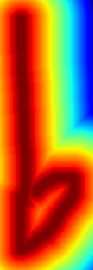
\includegraphics[height=5cm]{gfx/techniques/scoring/flats/6193-distance.png}
        \caption{Distance}
    \end{subfigure}
    \begin{subfigure}[b]{.19\linewidth}
        \centering
        
\includegraphics[height=5cm]{gfx/techniques/scoring/flats/6193-watershed.png}
        \caption{Watershed}
        \label{fig:flat-broken-watershed}
    \end{subfigure}
    \begin{subfigure}[b]{.19\linewidth}
        \centering
        
\includegraphics[height=5cm]{gfx/techniques/scoring/flats/6193-segmented.png}
        \caption{Merged}
        \label{fig:flat-broken-merged}
    \end{subfigure}
    \begin{subfigure}[b]{.19\linewidth}
        \centering
        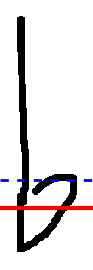
\includegraphics[height=5cm]{gfx/techniques/scoring/flats/6193-center.png}
        \caption{Centre}
    \end{subfigure}

  \caption{Identifying flat centre with watershed segmentation}
  \label{fig:flats-centre-watershed}
\end{figure}

An alternative solution uses dilations. This involves expanding the drawn image (and consequently shrinking the flat's `head' region) evenly until a distinct island region is formed (\cref{fig:flat-dilation}). Once that happens the vertical centre of the `head' can be established in the same way as outlined previously, using the centroid.

\begin{figure}[H]
    \centering
    \begin{subfigure}[b]{.2\linewidth}
        \centering
        
\includegraphics[height=5cm]{gfx/techniques/scoring/flats/6193-dilation-original.png}
        \caption{Original}
    \end{subfigure}
    \begin{subfigure}[b]{.2\linewidth}
        \centering
        
\includegraphics[height=5cm]{gfx/techniques/scoring/flats/6193-dilation-dilated.png}
        \caption{Dilation}
        \label{fig:flat-dilation}
    \end{subfigure}
    \begin{subfigure}[b]{.2\linewidth}
        \centering
        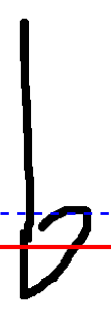
\includegraphics[height=5cm]{gfx/techniques/scoring/flats/6193-dilation-center}
        \caption{Centre}
    \end{subfigure}

  \caption{Identifying flat centre with dilation and connected component segmentation}
  \label{fig:flats-centre-dilation}
\end{figure}

\subsubsection{Note Head Centres}

For note heads, it was discovered that the centroid was a good representation of the centre, even in case of broken minims as seen in \cref{fig:broken-minim}

\begin{figure}[H]
    \centering
    \begin{subfigure}[b]{.32\linewidth}
        \centering
        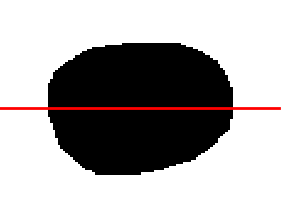
\includegraphics[width=\linewidth]{gfx/techniques/scoring/note-head/1906-centroid-centre.png}
        \caption{Crotchet Head}
    \end{subfigure}
    \begin{subfigure}[b]{.32\linewidth}
        \centering
        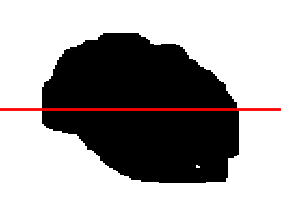
\includegraphics[width=\linewidth]{gfx/techniques/scoring/note-head/6189-centroid-centre.png}
        \caption{Wonky Crotchet Head}
    \end{subfigure}
    \begin{subfigure}[b]{.32\linewidth}
        \centering
        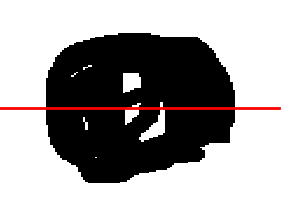
\includegraphics[width=\linewidth]{gfx/techniques/scoring/note-head/6192-centroid-centre.png}
        \caption{Inconsistent Crotchet Head}
    \end{subfigure}

    \begin{subfigure}[b]{.3\linewidth}
        \centering
        \includegraphics[width=\linewidth]{gfx/techniques/scoring/note-head/1818-centroid-centre.png}
        \caption{Minim Head}
    \end{subfigure}
    \begin{subfigure}[b]{.3\linewidth}
        \centering
        \includegraphics[width=\linewidth]{gfx/techniques/scoring/note-head/6105-centroid-centre.png}
        \caption{Broken Minim Head}
        \label{fig:broken-minim}
    \end{subfigure}

  \caption{Filled and hollow note heads with their centres identified by two red intersecting lines}
  \label{fig:ccl-two-pass}
\end{figure}

\subsection{Duration}
\label{sec:duration-identification}

There are two main steps to the process for calculating note duration. The first is the extraction of the fundamental note value, is it a semibreve, minim, crotchet, quaver or semiquaver? For a  semibreve, the note value will always be four, however for other notes, things are not so straightforward.

We first examine each note individually to ascertain the components which make up the note duration and then assign it a base value. For example we are particularly interested in the note head (is it solid or hollow?) and any tails or beaming. An outline of this heuristic can be seen in \cref{fig:note-duration-flow-chart}.

The number of tails is fairly straightforward as they are attached to isolated notes or are they joined in a more complex beam such as that in \cref{fig:complex-beam-establish}. however, we need to have some way to work out which notes have which values. To do this, a section the width of $\text{Stave Space} / 2$ is examined either side of the note's head. The beam is analysed in these segments for the maximum number of vertical black runs which represents the number beams.

\begin{figure}[H]
  \includegraphics[width=\linewidth]{gfx/implementation/beam-identification.png}
  \caption{Calculating the number of beams to get note values. Blue areas show the regions scanned and green lines represent the maximum count of vertical black runs found}
  \label{fig:complex-beam-establish}
\end{figure}

\begin{figure}[H]
  \includegraphics[width=\linewidth]{gfx/implementation/duration-diagram.png}
  \caption{Flow chart for establishing base note duration}
  \label{fig:note-duration-flow-chart}
\end{figure}

Note that with regards to tails and beaming, since every additional beam or tail present for the note divides it's value by two (examples can be seen in \cref{table:note-lengths}) we can generalise this section of the heuristic to deal with any number of beams and tails.

An example of a manuscript where the basic durations have been calculated can be seen in \cref{fig:canvas-durations}

\begin{figure}[hbt]
  \includegraphics[width=\linewidth]{gfx/techniques/labelling/duration.png}
  \caption{The manuscript after component duration analysis}
  \label{fig:canvas-durations}
\end{figure}

Once the base value has been obtained, we perform a final check of the area surrounding the note centre for any `modifier' dots. These extend the duration of the note by half, so for example, a dotted crotchet would last 1.5 beats as opposed to 1 beat without the dot. The region searched equates to half a staff space down and either side of the note as shown in \cref{fig:identify-dot}, anything outside of this region is ignored.

\begin{figure}[H]
  \includegraphics[width=\linewidth]{gfx/implementation/dot-identification.png}
  \caption{Searching for dots which would modify a note's length. Blue areas are the searched space for each note}
  \label{fig:identify-dot}
\end{figure}

\subsection{Domain Knowledge}
\label{sec:identification-domain-knowledge}

After all the segmentation, classification, pitch and duration analysis we can use domain knowledge as outlined in \cref{sec:arebelo-domain-knowledge,sec:domain-knowledge-taubman} to apply musical rules (with looser thresholds and variations in control flow to account for the potential mistakes like those in \cref{sec:common-manuscript-mistakes}) to group components as seen in \cref{fig:canvas-domain-knowledge}, enabling scoring \cref{sec:scoring} of the manuscript.

\begin{figure}[hbt]
  \includegraphics[width=\linewidth]{gfx/techniques/labelling/domain-knowledge.png}
  \caption{The manuscript after application of domain knowledge. Note the time signature, key signature and clef components have been grouped correctly}
  \label{fig:canvas-domain-knowledge}
\end{figure}

\section{Scoring}

\subsection{Key Signatures}
\todo[inline,color=red]{Scoring Techniques - Key Signatures}

\subsection{Beats and Timing}
\todo[inline,color=red]{Scoring Techniques - Beats and Timing}

\subsection{Stem Straightness}

Given a drawn note stem, we wish to be able to determine a measure of `straightness' which we can threshold to discern a badly drawn stem shown in \cref{fig:wonky-stems} from a straight one  as shown in \cref{fig:straight-stems}.

\begin{figure}[h!]
    \centering
    \begin{subfigure}[b]{.4\linewidth}
        \centering
        \includegraphics[height=4cm]{gfx/implementation/stem-straightness/4912.png}
        \quad
        \includegraphics[height=4cm]{gfx/implementation/stem-straightness/5371.png}
        \caption{Examples of uneven stems}
        \label{fig:wonky-stems}
    \end{subfigure}
    \begin{subfigure}[b]{.4\linewidth}
        \centering
        \includegraphics[height=4cm]{gfx/implementation/stem-straightness/3876.png}
        \quad
        \includegraphics[height=4cm]{gfx/implementation/stem-straightness/5104.png}
        \caption{Examples of straight stems}
        \label{fig:straight-stems}
    \end{subfigure}

    \caption{Examples of straight and uneven stems}
    \label{fig:stem-straightness-examples}
\end{figure}

Stem straightness is different to the stem angle because intuitively even if the stem is angled, it can still be straight. Therefore, we need to establish a technique which gives a measure irrespective of the stem angle.

To do this, we take the original stem (\cref{fig:straight-skeleton-original}) and generate it's skeletal representation using techniques outlined in \cref{sec:skeletonization} which approximates a line following the center of the stem (\cref{fig:straight-skeleton-skeleton}). If we treat this skeleton as a plot of points, we can draw a line of best fit through them to approximate what a perfectly straight version of the stem (\cref{fig:straight-skeleton-bestfit}).

\begin{figure}[h!]
    \centering

    \begin{subfigure}[b]{.3\linewidth}
        \centering
        \frame{\includegraphics[height=3cm]{gfx/techniques/skeletonization/4705.png}}
        \frame{\includegraphics[height=3cm]{gfx/techniques/skeletonization/4912.png}}
        \caption{Original}
        \label{fig:straight-skeleton-original}
    \end{subfigure}
    \begin{subfigure}[b]{.3\linewidth}
        \centering
        \frame{\includegraphics[height=3cm]{gfx/techniques/skeletonization/4705_skeleton.png}}
        \frame{\includegraphics[height=3cm]{gfx/techniques/skeletonization/4912_skeleton.png}}
        \caption{Skeleton}
        \label{fig:straight-skeleton-skeleton}
    \end{subfigure}
    \begin{subfigure}[b]{.3\linewidth}
        \centering
        \frame{\includegraphics[height=3cm]{gfx/techniques/skeletonization/4705_bestfit.png}}
        \frame{\includegraphics[height=3cm]{gfx/techniques/skeletonization/4912_bestfit.png}}
        \caption{Best Fit}
        \label{fig:straight-skeleton-bestfit}
    \end{subfigure}

    \caption{Examples of stem skeletons}
    \label{fig:stem-skeletons}
\end{figure}

We now have a skeleton line \cref{eqn:l-skeleton} and a best fit line \cref{eqn:l-ref} we can calculate the difference at each point \cref{eqn:l-residuals}.

\begin{equation} \label{eqn:l-skeleton}
    L_{\text{skeleton}}(x) = (a_0, a_1, a_2, \ldots, a_n)
\end{equation}
\begin{equation} \label{eqn:l-ref}
    L_{\text{ref}}(x) = (b_0, b_1, b_2, \ldots, b_n)
\end{equation}
\begin{equation} \label{eqn:l-residuals}
    R(x) = (r_0, r_1, r_2, \ldots, r_n), r_i = a_i - b_i)
\end{equation}


After experimenting with using the standard deviation \cref{eqn:sd} of the residuals as the straightness measure the results turned out to be positive upon visual inspection. As you can see in \cref{fig:stem-straightness-ranking} when ranked according to their `straightness' measure, the stems do indeed appear to be ordered according to what one would visually define as being `straight'.

\begin{equation} \label{eqn:sd}
\sigma = \sqrt{\frac{\sum\limits_{i=1}^{n}\left(r_{i} - \bar{r}\right)^{2}}{n-1}}
\end{equation}


\begin{figure}[h!]
  \centering
  \tiny
  \captionsetup[subfigure]{labelformat=empty}

  \subcaptionbox{7.3\label{fig:stem-straightness-4912}}[0.04\linewidth]{
    \includegraphics[height=1.5cm,keepaspectratio]{gfx/implementation/stem-straightness/4912.png}
  }
  \subcaptionbox{3.3\label{fig:stem-straightness-3889}}[0.04\linewidth]{
    \includegraphics[height=1.5cm,keepaspectratio]{gfx/implementation/stem-straightness/3889.png}
  }
  \subcaptionbox{3.1\label{fig:stem-straightness-4064}}[0.04\linewidth]{
    \includegraphics[height=1.5cm,keepaspectratio]{gfx/implementation/stem-straightness/4064.png}
  }
  \subcaptionbox{2.7\label{fig:stem-straightness-5371}}[0.04\linewidth]{
    \includegraphics[height=1.5cm,keepaspectratio]{gfx/implementation/stem-straightness/5371.png}
  }
  \subcaptionbox{2.5\label{fig:stem-straightness-3796}}[0.04\linewidth]{
    \includegraphics[height=1.5cm,keepaspectratio]{gfx/implementation/stem-straightness/3796.png}
  }
  \subcaptionbox{2.4\label{fig:stem-straightness-3845}}[0.04\linewidth]{
    \includegraphics[height=1.5cm,keepaspectratio]{gfx/implementation/stem-straightness/3845.png}
  }
  \subcaptionbox{2.2\label{fig:stem-straightness-4055}}[0.04\linewidth]{
    \includegraphics[height=1.5cm,keepaspectratio]{gfx/implementation/stem-straightness/4055.png}
  }
  \subcaptionbox{1.8\label{fig:stem-straightness-4072}}[0.04\linewidth]{
    \includegraphics[height=1.5cm,keepaspectratio]{gfx/implementation/stem-straightness/4072.png}
  }
  \subcaptionbox{1.6\label{fig:stem-straightness-4758}}[0.04\linewidth]{
    \includegraphics[height=1.5cm,keepaspectratio]{gfx/implementation/stem-straightness/4758.png}
  }
  \subcaptionbox{1.5\label{fig:stem-straightness-4653}}[0.04\linewidth]{
    \includegraphics[height=1.5cm,keepaspectratio]{gfx/implementation/stem-straightness/4653.png}
  }
  \subcaptionbox{1.4\label{fig:stem-straightness-4183}}[0.04\linewidth]{
    \includegraphics[height=1.5cm,keepaspectratio]{gfx/implementation/stem-straightness/4183.png}
  }
  \subcaptionbox{1.2\label{fig:stem-straightness-4250}}[0.04\linewidth]{
    \includegraphics[height=1.5cm,keepaspectratio]{gfx/implementation/stem-straightness/4250.png}
  }
  \subcaptionbox{1.1\label{fig:stem-straightness-4003}}[0.04\linewidth]{
    \includegraphics[height=1.5cm,keepaspectratio]{gfx/implementation/stem-straightness/4003.png}
  }
  \subcaptionbox{0.9\label{fig:stem-straightness-5350}}[0.04\linewidth]{
    \includegraphics[height=1.5cm,keepaspectratio]{gfx/implementation/stem-straightness/5350.png}
  }
  \subcaptionbox{0.8\label{fig:stem-straightness-4103}}[0.04\linewidth]{
    \includegraphics[height=1.5cm,keepaspectratio]{gfx/implementation/stem-straightness/4103.png}
  }
  \subcaptionbox{0.7\label{fig:stem-straightness-5104}}[0.04\linewidth]{
    \includegraphics[height=1.5cm,keepaspectratio]{gfx/implementation/stem-straightness/5104.png}
  }
  \subcaptionbox{0.6\label{fig:stem-straightness-4038}}[0.04\linewidth]{
    \includegraphics[height=1.5cm,keepaspectratio]{gfx/implementation/stem-straightness/4038.png}
  }
  \subcaptionbox{0.5\label{fig:stem-straightness-4565}}[0.04\linewidth]{
    \includegraphics[height=1.5cm,keepaspectratio]{gfx/implementation/stem-straightness/4565.png}
  }
  \subcaptionbox{0.4\label{fig:stem-straightness-4011}}[0.04\linewidth]{
    \includegraphics[height=1.5cm,keepaspectratio]{gfx/implementation/stem-straightness/4011.png}
  }
  \subcaptionbox{0.3\label{fig:stem-straightness-3327}}[0.04\linewidth]{
    \includegraphics[height=1.5cm,keepaspectratio]{gfx/implementation/stem-straightness/3327.png}
  }
  \subcaptionbox{0.2\label{fig:stem-straightness-4752}}[0.04\linewidth]{
    \includegraphics[height=1.5cm,keepaspectratio]{gfx/implementation/stem-straightness/4752.png}
  }
  \subcaptionbox{0.1\label{fig:stem-straightness-3876}}[0.04\linewidth]{
    \includegraphics[height=1.5cm,keepaspectratio]{gfx/implementation/stem-straightness/3876.png}
  }
  \caption{Ranking of stems according to their `straightness' score}
  \label{fig:stem-straightness-ranking}
\end{figure}


\subsection{Stem Angle}

In order to determine the angle of a stem, we first need establish the line of best fit which most accurately reflects the direction of the stem, we can then examine this line $y = mx + c$ and compute $\arctan(m)$ to get the angle relative to vertical.

\begin{figure}[h!]
    \centering

    \begin{subfigure}[b]{.45\linewidth}
        \centering
        \frame{\includegraphics[height=6cm]{gfx/techniques/skeletonization/4705.png}}
        \caption{Original}
    \end{subfigure}
    \begin{subfigure}[b]{.45\linewidth}
        \centering
        \frame{\includegraphics[height=6cm]{gfx/techniques/skeletonization/4705_bestfit_angle.png}}
        \caption{Best fit line with angle calculation}
    \end{subfigure}

    \caption{Examples of stem skeletons}
    \label{fig:stem-skeletons}
\end{figure}

 \begin{figure}[h!]
        \centering
        \tiny
        \addtolength{\subfigcapskip}{0.2cm}

        \subfigure[-23.9]{
          \includegraphics[height=2cm,keepaspectratio]{gfx/implementation/stem-angle/4883.png}
          \label{fig:stem-angle-4883}
        }
        \quad
        \subfigure[-20.0]{
          \includegraphics[height=2cm,keepaspectratio]{gfx/implementation/stem-angle/4718.png}
          \label{fig:stem-angle-4718}
        }
        \quad
        \subfigure[18.7]{
          \includegraphics[height=2cm,keepaspectratio]{gfx/implementation/stem-angle/4705.png}
          \label{fig:stem-angle-4705}
        }
        \quad
        \subfigure[-14.7]{
          \includegraphics[height=2cm,keepaspectratio]{gfx/implementation/stem-angle/4886.png}
          \label{fig:stem-angle-4886}
        }
        \quad
        \subfigure[-9.8]{
          \includegraphics[height=2cm,keepaspectratio]{gfx/implementation/stem-angle/4892.png}
          \label{fig:stem-angle-4892}
        }
        \quad
        \subfigure[-8.4]{
          \includegraphics[height=2cm,keepaspectratio]{gfx/implementation/stem-angle/4645.png}
          \label{fig:stem-angle-4645}
        }
        \quad
        \subfigure[7.3]{
          \includegraphics[height=2cm,keepaspectratio]{gfx/implementation/stem-angle/3889.png}
          \label{fig:stem-angle-3889}
        }
        \quad
        \subfigure[6.2]{
          \includegraphics[height=2cm,keepaspectratio]{gfx/implementation/stem-angle/5380.png}
          \label{fig:stem-angle-5380}
        }
        \quad
        \subfigure[5.1]{
          \includegraphics[height=2cm,keepaspectratio]{gfx/implementation/stem-angle/4194.png}
          \label{fig:stem-angle-4194}
        }
        \quad
        \subfigure[-4.1]{
          \includegraphics[height=2cm,keepaspectratio]{gfx/implementation/stem-angle/3970.png}
          \label{fig:stem-angle-3970}
        }
        \quad
        \subfigure[3.0]{
          \includegraphics[height=2cm,keepaspectratio]{gfx/implementation/stem-angle/4783.png}
          \label{fig:stem-angle-4783}
        }
        \quad
        \subfigure[2.0]{
          \includegraphics[height=2cm,keepaspectratio]{gfx/implementation/stem-angle/3920.png}
          \label{fig:stem-angle-3920}
        }
        \quad
        \subfigure[-1.0]{
          \includegraphics[height=2cm,keepaspectratio]{gfx/implementation/stem-angle/5368.png}
          \label{fig:stem-angle-5368}
        }
        \quad

        \caption{Ranking of stems according to their off-vertical angle}
        \label{fig:stem-angle-ranking}
      \end{figure}




\subsection{Stem Direction}

To establish the stem direction which I will refer to as $S_d$, the vertical position (y coordinates) of the head and the stem are compared.

If the stem is located at $(x_{\text{stem}}, y_{\text{stem}})$ and the note head at $(x_{\text{head}}, y_{\text{head}})$, knowing that the coordinate axes have an origin starting from the top right of a given image, we can establish the following classifications:

$$
S_{d} (y_{\text{stem}}, y_{\text{head}}) =
\left\{
	\begin{array}{ll}
		\text{up}   & \mbox{if } y_{\text{stem}} < y_{\text{head}} \\
		\text{down} & \mbox{if } y_{\text{stem}} > y_{\text{head}}
	\end{array}
\right.
$$

The case where a stem has the same $y$ coordinate as it's head isn't possible due to the way stems are extracted from a note complex as for this to happen a stem would need to be extracted \emph{out} of a note head. Since note heads are removed in order to identify stems as in \todo[color=blue]{REFERENCE: Extracting Stems}, this is impossible.

\begin{table}[h]

    \begin{tabularx}{\textwidth}{ X l l l l }
    \toprule
    Component & Stem Y   & Head Y   & Predicted Direction & True Direction \\
    \midrule
    \bottomrule
    \end{tabularx}

    \label{table:stem-direction-results}
    \caption{Results of the stem direction classification heuristic}
\end{table}
\todo[inline,color=purple]{Stem Direction: Results Table (Showing stems and classification of up/down)}



\subsection{Stem Side}
To establish the stem side which I will refer to as $S_s$, we do a similar operation to in determining the direction, however, since it is perfectly feasible that the stem and head have the same x coordinate, we can't just use the x coordinate directly.

Instead, we compare the x coordinate of the stem $x_{\text{stem}}$ to the true centre \todo{Better definition later please} of the note head $cx_{\text{head}}$

Again, given that the coordinate axes start from the top left, we can now establish the stem x offset

$$
S_\text{xoff} = x_{\text{stem}} - cx_{\text{head}}
$$

Using this, we can establish the side classification as
$$
S_{s} (S_\text{xoff}) =
\left\{
	\begin{array}{ll}
		\text{left}   & \mbox{if } S_\text{xoff} < 0 \\
		\text{right}  & \mbox{if } S_\text{xoff} \ge 0
	\end{array}
\right.
$$

\subsection{Stem Length}

Stem length may seem like a simple case of measuring the length of the extracted stem, but it's actually a little more complicated. In order to get the best results, we need to take into account the fact that the stem has been extracted from the note head and that this separation point could occur anywhere from near the bottom to the top as shown in \cref{fig:stem-intersection}.

\begin{figure}[h!]
    \centering
    \includegraphics[width=.8\textwidth]{gfx/techniques/stem-intersection-labelled.png}
    \caption{An example of the effect stem and note head intersection can have on length. Note that the right hand note would, if the raw stem was extracted, have a longer stem (potentially perceived as \emph{too} long) but in actual fact both stems reach the required height}
    \label{fig:stem-intersection}
\end{figure}

Similarly to the straightness and angular measures, we can establish the raw length $L_R$ by drawing a line through the perceived centre of the stem and measuring it's length using simple trigonometry. However, although it might seem counterintuitive to not use this as a measure of length, in reality a better measure of whether the stem is `too long' is to measure the distance between the stave line/space above stem's associated notehead and the y coordinate of the stem.

If we define the correct length $L_E$ for a stem as outlined in \todo{REFERENCE where I talk about correct stem length} then the length score is therefore just $L_E - L_A$ where smaller values mean the stem is closer to the expected length.

\subsection{Quaver Tail Side}

\todo[inline]{Quaver tail side needs a little more detail, this feels a bit 'late in the evening' weak. Also, MORE MATHS}

To determine on which side a quaver tail lies, left (\cref{fig:quaver-tail-left}) or right (\cref{fig:quaver-tail-right}), intially I attempted to utilise vertical projections, much as in segmentation (\cref{sec:projections}).

\begin{figure}[h!]
    \centering

    \begin{subfigure}[b]{.45\linewidth}
        \centering
      \includegraphics[height=5cm]{gfx/techniques/quaver-left-6087.png}
      \caption{A left sided quaver tail}
      \label{fig:quaver-tail-left}
    \end{subfigure}
    \begin{subfigure}[b]{.45\linewidth}
        \centering
      \includegraphics[height=5cm]{gfx/techniques/quaver-right-3083.png}
      \caption{A right sided quaver tail}
      \label{fig:quaver-tail-right}
    \end{subfigure}
    
\end{figure}

After taking a vertical projection of the quaver tail, the maximum peak in the projection is taken and by establishing on which side of the centre the peak lies, this told us which side the `flick' of the quaver is on.

However, occasionally a quaver tail would be encountered where the distinction wasn't very clear \todo[color=purple]{Example of non-distinct quaver tail position}.

Another method I investigated was to divide the image into two horizontally, then calculate the average black pixel column coordinate in each half as seen in \cref{fig:quaver-tail-average-position}. By working out which half has the highest average pixel position, we can then establish the side on which the tail lies.

% Generate the below with: python reporting_quavertail.py 3811
\begin{figure}[h!]
    \centering

    \begin{subfigure}[b]{.45\linewidth}
        \centering
      \frame{\includegraphics[height=7cm]{gfx/techniques/quaver-pixel-average-right.png}}
      \caption{Identifying a right sided tail}
      \label{fig:quaver-tail-average-position-right}
    \end{subfigure}
    \begin{subfigure}[b]{.45\linewidth}
        \centering
      \frame{\includegraphics[height=7cm]{gfx/techniques/quaver-pixel-average-left}}
      \caption{Identifying a left sided tail}
      \label{fig:quaver-tail-average-position-left}
    \end{subfigure}
    
      \caption{Calculating the quaver tail position with pixel averages}
      \label{fig:quaver-tail-average-position}
\end{figure}

\subsection{Note Heads}
\todo[inline,color=red]{Scoring Techniques - Note Head - Filled Percentage?? (ambiguity)}
\todo[inline,color=red]{Scoring Techniques - Note Head - Gaps/broken circles}
\todo[inline,color=red]{Scoring Techniques - Note Head - Eccentricity?}

\section{Feedback}

\subsection{Listing Mistakes}
\label{sec:feedback-listing}
\todo[inline,color=red]{Feedback Techniques - List of Issues}

- Very clear what's wrong

- Comes across negative

- Doesn't necessarily help them know what to do next time

- Easy to generate

- Didn't always mean much to the child

\subsection{Colour Coding}
\todo[inline,color=red]{Feedback Techniques - List of Issues}

- Nice and visual

- Can highlight component by component (perhaps in conjunction with \cref{sec:feedback-listing}

- Traffic Light system

- Didn't always mean much to the child

\subsection{On Screen Correction}

- Scaling, Rotation, Translation

- Animations were very clear :)

- Hard to do! Lots of potential difficulties

- Child immediately got what they'd done wrong

\subsection{Aggregation}
Given the large number of scoring results given for a manuscript drawing, some of the early testers suggested that a simple scoring system could be used like stars from 1 to 3 or 1 to 5.

To produce a simple numeric score we must somehow aggregate the more detailed feedback. For example, by assigning weights to `musical correctness', `stems', `note heads' etc, we can produce a score in a reasonable range for overall feedback in a more simplistic form.

\begin{figure}[H]
  \includegraphics[width=\linewidth]{gfx/photos/user-receiving-feedback.jpg}
  \caption{Child receiving simplified graphical feedback}
\end{figure}


\chapter{Implementation}

\section{Architecture}

\todo[inline,color=red]{Implementation Architecture}

Entity diagrams of whole system, then of front end and back end separately
\section{Medium Selection}
\label{sec:medium-selection}

The first step in this project was to establish the best method for a student to interact with the application. As seen in \cref{sec:prior-research} a lot of different mediums for OMR have been tried over the years, however which one would be most suitable for student use wouldn't necessarily correlate with which was best for quality of scanning, speed of analysis etc.

\subsection{Flat Bed Scanner}

The most simple of all the input methods, this would involve a student writing on a sheet of manuscript paper, then using a flat bed scanner (the type commonly found as a standalone device and in multi-function printers) to input the sheet into the computer. This method allows for a scan with high and consistent light levels (minimising noise and light-dependent artefacts), minimal distortion due to paper curvature (as the scanner usually flattens the sheet) and a high resolution end image, typically 300-600dpi.

The application would process the sheet using traditional OMR techniques and then provide feedback to the student. This technique would therefore require ownership of both a scanner and a computer on which to install and run the application. Alternatively, the student could upload the scanned image to a web based service for analysis, removing the need to install software.

\subsection{Photograph/Camera}

Total free for all, colours and light levels vary, extraction from background, resolution variable, noise variable

Project 8 Final Report

\subsection{Gestures}

Use gestures combined with classification (see book and some papers).
Good for classifying individual entities but more like the old palm tablets, usually one note at a time


\subsection{Tablet Input}

Finger difficult, stylus better, not always available

\subsection{Comparison Matrix}

\section{Input}

\subsection{Medium Selection}
\label{sec:medium-selection}

The first step in this project was to establish the best method for a student to interact with the application. As seen in \cref{sec:prior-research} a lot of different mediums for OMR have been tried over the years, however which one would be most suitable for a student to use wouldn't necessarily correlate with which was best for quality of scanning, speed of analysis etc.

\subsubsection{Flat Bed Scanner}

The most simple of all the input methods, this would involve a student writing on a sheet of manuscript paper, then using a flat bed scanner (the type commonly found as a standalone device and in multi-function printers) to input the sheet into the computer. This method allows for a scan with high and consistent light levels (minimising noise and light-dependent artefacts), minimal distortion due to paper curvature (as the scanner usually flattens the sheet) and a high resolution end image, typically 300-600dpi.

The application would process the sheet using traditional OMR techniques and then provide feedback to the student. This technique would therefore require ownership of both a scanner and a computer on which to install and run the application. Alternatively, the student could upload the scanned image to a web based service for analysis, removing the need to install software.

\subsubsection{Photograph/Camera}

\todo[inline,color=red]{Implementation - Photo/Camera}

Total free for all, colours and light levels vary, extraction from background, resolution variable, noise variable

Reference `Project 8 Final Report'

\subsubsection{Gestures}
\todo[inline,color=red]{Implementation - Gestures}

Use gestures combined with classification (see book and some papers).
Good for classifying individual entities but more like the old palm tablets, usually one note at a time

\subsubsection{Tablet Input}
\todo[inline,color=red]{Implementation - Tablet Input}

Finger or stylus work well tends to depend on the child, finger often felt more natural

\begin{figure}[h!]
    \centering
    \begin{subfigure}[b]{.49\linewidth}
        \centering
        \includegraphics[width=\linewidth]{gfx/photos/user-finger.jpg}
        \caption{Using a finger}
    \end{subfigure}
    \begin{subfigure}[b]{.49\linewidth}
        \centering
        \includegraphics[width=\linewidth]{gfx/photos/user-stylus.jpg}
        \caption{Using a stylus}
    \end{subfigure}

    \caption{Examples of a student trying different tablet input methods}
\end{figure}

Chose this method in the end


\subsection{Capturing Strokes}
\label{sec:capturing-strokes}
To capture strokes drawn by the user, several listeners are attached to the HTML5 canvas element on which the manuscript is rendered. When the user presses their mouse down or initiates a touch event, a new array of line points is created and the initial point of interaction is stored in that array. From there, any mouse or touch movement whilst the touch or `mousedown' event is active triggers a new point recording, until the mouse button is released or the touch event ends. In this way, an array of points is built up which represent a drawn line.

Each time the line changes via the addition of new points, a redraw event is triggered which connects all the points together and renders the line onto the canvas.

In initial experiments with simple manuscript entities, this worked well, however as children began to experiment with more complex entities (requiring more lines and therefore more points) the length of time required to redraw the lines on the canvas became prohibitively long. Eventually a lag occurred between `pen' movement and lines being rendering on the canvas, the result of which was that as more lines were drawn, the time between new points being registered increased. This increase led to the drawing experience feeling (as one user described it) `really clunky' and long straight lines appearing instead of smooth curves (\cref{fig:drawing-lag-rough}).

\begin{figure}[hbt                                   ]
    \centering

    \begin{subfigure}[b]{.49\linewidth}
        \centering
      \includegraphics[width=\linewidth]{gfx/implementation/lag-stave.png}
      \caption{Drawing with refresh rendering - note that after drawing a high density region of many points, a spiral outward is very `angular' due to the additional time it takes to redraw so many points on every movement event }
      \label{fig:drawing-lag-rough}
    \end{subfigure}
    \begin{subfigure}[b]{.49\linewidth}
        \centering
      \includegraphics[width=\linewidth]{gfx/implementation/nolag-stave.png}
      \caption{Drawing with incremental rendering, not that after a similar high density region of points, the curve outwards still appears smooth}
      \label{fig:drawing-lag-smooth}
    \end{subfigure}

  \label{Drawing Lag}

\end{figure}

To counteract this, I modified the code such that it renders new line segments on the fly, rather than re-rendering all the lines every time a new point is added. Although this requires some more logic to render the line segment, but overall the experience turned out much smoother as the small increase in the length of the code path had much less impact than re-rendering the drawing every time (\cref{fig:drawing-lag-smooth}).

\section{Data Storage and Retrieval}

\subsection{Stave Drawing}
I store the data gathered in \cref{sec:capturing-strokes} in two ways.

Firstly, I store the serialized JSON of the stroke data in the database. This enables potential later on to experiment more with gesture based segmentation and recognition \todo[inline]{Reference Gesture based recognition}, showing a student corrections by transforming points in the strokes as opposed to transformations on the image. It also facilitates some great UI features like playing back the drawing for the tutor so they can see exactly how the student approached the problem and more ideas I express in \cref{sec:future-work}.

Secondly, I store the entire rendered canvas in the cloud using an Amazon S3 bucket, as a 'reference copy' in case I need to check the JSON against the original image at a later date or re-analyse images after updating my classifiers, features or analysis techniques.

\todo[inline]{Should I show my database schema here?}

\subsection{Components}

Once components have been extracted from the drawing using the techniques outlined in \cref{sec:identification}, I store both their features and \acrfull{RLE} representation of the whole component in the database for retrieval later during any further image processing.

Although 3000 components uses around 1GB in data when raw, using compression we are able to lower this considerably using run length encoding as shown in \ref{table:rle-improvement}.

\begin{table}[H]

    \begin{tabularx}{\textwidth}{ X X X X }
    \toprule
    Metric                  & Without RLE   & With RLE   & Improvement \\
    \midrule
    Storage Required        & 759 MB        & 22 MB      & 91.7\%      \\
    Total Retrieval Time    & 1639 ms       & 42 ms      & 97.4\% \\
    \bottomrule
    \end{tabularx}

    \caption{To improve the speed of my application, I utilised \acrfull{RLE} (covered in \cref{sec:tb-rle}) to improve storage and retrieval times during feature extraction and classification by up to 97\% (\cref{table:rle-improvement}).}
    \label{table:rle-improvement}
\end{table}

\subsection{Database Schema}

\subsection{Entity Relationship Diagram}







\section{Feedback}

\chapter{Evaluation}

\section{Mistake Detection}

\begin{quotation}
\emph{Objective}: Enable the detection of common errors in notation symbols, pitch, time signatures and other musical features outlined in \cref{table:teacher-feedback-summary}.
\end{quotation}

This is one of the most important evaluation components, can we in fact spot the same mistakes which a teacher would?

I short, yes, I believe we can and although long term data gathering and trials haven't been performed, preliminary data is positive.

Once the likely mistakes had been established (\cref{table:teacher-feedback-summary}), I developed an application which assisted in rapid assignment of relevant mistakes to score entities by a human, shown in more detail in \cref{sec:implementation-mistake-classification}. I also used this over the original data gathered from students and ongoing data from participants and experiments.

The result was a database of entities and their mistakes which I then used to adjust thresholds and parameters in \cref{sec:scoring}. It would be interesting to modify these values according to the results of scoring against this database automatically and I talk more about this in \cref{sec:future}.

By comparing my heuristics against the `true' data provided by professionals and competent musicians I generated confusion matrices for each of the mistakes.

The full dataset of results for the implemented mistake heuristics and algorithms can be seen in \cref{table:results-matrix}. Motice that for the majority of mistakes, we obtain a great accuracy, however since most samples actually do \emph{not} get labelled with a mistake, the accuracy is unfairly weighted by the large number of true negatives, meaning it isn't necessarily the best performance criteria. Instead, I think that it makes more sense to judge our system by it's predictive power or \emph{Precision} (the proportion of predicted positives which are actually positives). If we do this, the results still appear successful


  \begin{figure}
    \centering
    \begin{subtable}[b]{\linewidth}
      \begin{tabularx}{\textwidth}{r | XXXXXX}
                                  & TP & FP & TN & FN & Accuracy & Precision \\
        \midrule
              note-head-ambiguous & 11 & 2& 251& 0 & 0.992 & 0.846 \\
                 note-head-broken & 24 & 1& 239& 0 & 0.996 & 0.96 \\
                 note-head-angled & 0 & 0& 256& 8 & 0.97 & NaN \\
                  note-head-messy & 7 & 0& 252& 5 & 0.981 & 1.0 \\
                note-head-too-big & 20 & 3& 241& 0 & 0.989 & 0.87 \\
              note-head-too-small & 8 & 0& 250& 6 & 0.977 & 1.0 \\
                stem-length-short & 17 & 7& 240& 0 & 0.973 & 0.708 \\
                 stem-length-long & 19 & 9& 236& 0 & 0.966 & 0.679 \\
                stem-straightness & 0 & 0& 245& 19 & 0.928 & NaN \\
             stem-direction-wrong & 11 & 6& 247& 0 & 0.977 & 0.647 \\
                  stem-side-wrong & 14 & 9& 241& 0 & 0.966 & 0.609 \\
                       stem-angle & 21 & 17& 224& 2 & 0.928 & 0.553 \\
                 quaver-tail-side & 0 & 0& 264& 0 & 1.0 & NaN \\
                   dot-wrong-side & 9 & 1& 254& 0 & 0.996 & 0.9 \\
            accidental-wrong-side & 19 & 4& 241& 0 & 0.985 & 0.826 \\
            accidental-wrong-line & 0 & 0& 264& 0 & 1.0 & NaN \\
                    keysig-octave & 0 & 3& 19& 0 & 0.864 & 0.0 \\
                     keysig-order & 0 & 1& 20& 1 & 0.909 & 0.0 \\
                keysig-wrong-clef & 0 & 0& 22& 0 & 1.0 & NaN \\
                 keysig-incorrect & 5 & 8& 9& 0 & 0.636 & 0.385 \\
             accidental-ambiguous & 0 & 0& 104& 0 & 1.0 & NaN \\
             accidental-ambiguous & 0 & 0& 104& 0 & 1.0 & NaN \\
                    rest-position & 0 & 0& 9& 0 & 1.0 & NaN \\

      \end{tabularx}
    \end{subtable}

    \caption{DATA BITCHES}
    \label{table:results-matrix}
  \end{figure}


\section{Notation Analysis}

\begin{quotation}
\emph{Objective}: Build a service which is capable of analysing a notation drawing and establishing one or more scores for multiple aspects of a notation attempt.
\end{quotation}

Notation analysis using computer vision and OMR techniques combined with Heuristics actually turned out to be quite successful in the end. As the results in \cref{sec:knn} show, we achieved a high level of accuracy for identification of musical symbols. Admittedly not as high as those of printed score OMR systems, but considering the data is handwritten and also comes in multiple often quite different representations, the model using KNN has perfomed rather well.

\subsection{Learning Improvement}

\begin{quotation}
\emph{Objective}: Produce an application which can improve on and continue a child's learning outside of lessons
\end{quotation}

This is one of the most difficult outcomes to measure, initial in person feedback and conversation with students after performing various notation tasks (such as those in \cref{sec:implementation-lessons} suggest that \noteED is doing a good job so far.

However, since a conversation is not a quantifiable measure of how well a child's learning has been improved, there is also logging throughout the system for use over a longer period of time, data such as average mistakes per task or mistakes compared to how many times a task has been done before can therefore be analysed. 

We propose that in order to best establish a reliable outcome for learning improvement, a minimum of one month's observation is needed and preferably closer in the region of 6 months if possible.

\subsection{Engaging Experience For Child}

\begin{quotation}
\emph{Objective}: Combine the tablet interface and notation analysis objectives to produce a streamlined experience which a student will happily engage with on a repeat basis.
\end{quotation}

Whilst talking with students was highly valuable in the design and implementation stages, what people say and what they do are often not the same\footnote{\url{http://www.nngroup.com/articles/first-rule-of-usability-dont-listen-to-users/}}. Therefore simply asking a student `would you use this again' isn't necessarily going to prove anything. Instead, we keep track of student actions and we can subsequently ascertain from these more reliable readings how often the student is interacting the the application.

Preliminary (gathered through in-person trials) data suggests that a student will happily perform a task 4-5 times before wanting to move on, usually because they got it right and got bored or in a few early cases, because the feedback and analysis wasn't being very helpful which was a useful discovery in itself.

\subsection{Tablet Interface}

\emph{Objective}: \\
A tablet oriented (or tablet compatible) user interface which can provide a child with simulated challenges around writing musical notation and easily allow them to input their attempts and display feedback.

\emph{Evaluation Technique}: \\
Verbal and written feedback from child on their experience using the tablet for input.

Verbal and written feedback from teachers on whether the tablet accurately reflects writing normal manuscript notation

\clearpage

\chapter{Conclusions}
\chapter{Future Work}\label{sec:future}

\begin{itemize}
  \item Horizontally scrolling manuscript
  \item Automatic theresholds for metrics
\end{itemize}

\clearpage

\chapter{Developer Guide}

In order to set up and run the \noteED application you will need to meet the following development requirements.

\section{Dependencies and libraries}
todo[inline,color=red]{Work in progress, finish before submission!}
\begin{itemize}
  \item Ruby running at v2.1.0 or higher
  \item Postgres
  \item nodeJS
  \item Node Package Manager
  \item imagemagick
  \item Python v2.7.5 or higher
  \item Scikit-image
  \item Scikit-learn
  \item all the other things
\end{itemize}


\section{Front End}

\begin{itemize}
  \item Written in Angular JS
  \item Split into pages etc
\end{itemize}


\section{Server}

\begin{itemize}
  \item Rails etc
\end{itemize}



\chapter{Appendices}
\begin{table}[H]

    \begin{tabularx}{\textwidth}{ lXXXXXXXXXX }
    \toprule
    & \multicolumn{10}{c}{Width (px)} \\
    \cmidrule{2-11}
    Height (px) & 10   & 20   & 30   & 40   & 50   & 60   & 70   & 80   & 90   & 100  \\
    \midrule
    10          & 0.948 & 0.961 & 0.955 & 0.954 & 0.962 & 0.953 & 0.951 & 0.953 & 0.955 & 0.957 \\
    20          & 0.947 & 0.963 & 0.963 & 0.962 & 0.964 & 0.962 & 0.956 & 0.961 & 0.960 & 0.966 \\
    30          & 0.945 & 0.960 & 0.954 & 0.965 & 0.958 & 0.958 & 0.956 & 0.958 & 0.959 & 0.959 \\
    40          & 0.946 & 0.968 & 0.957 & 0.963 & 0.958 & 0.950 & 0.961 & 0.964 & 0.960 & 0.966 \\
    50          & 0.935 & 0.969 & 0.965 & 0.957 & 0.961 & 0.957 & 0.967 & 0.959 & 0.948 & 0.962 \\
    60          & 0.953 & 0.971 & 0.960 & 0.963 & 0.962 & 0.967 & 0.948 & 0.957 & 0.957 & 0.963 \\
    70          & 0.954 & 0.970 & 0.969 & 0.960 & 0.974 & 0.960 & 0.957 & 0.956 & 0.960 & 0.969 \\
    80          & 0.959 & 0.962 & 0.959 & 0.964 & 0.963 & 0.965 & 0.957 & 0.963 & 0.963 & 0.954 \\
    90          & 0.954 & 0.961 & 0.958 & 0.960 & 0.956 & 0.959 & 0.963 & 0.959 & 0.963 & 0.956 \\
    100         & 0.955 & 0.967 & 0.965 & 0.963 & 0.958 & 0.960 & 0.960 & 0.965 & 0.960 & 0.962 \\
    \bottomrule
    \end{tabularx}

    \caption{Accuracy Matrix for various Height and Width Downsampling Combinations}
    \label{table:height-width-matrix}
\end{table}


\printbibliography

\glossarystyle{list}

\printglossary[type=\acronymtype] % prints just the list of acronyms
\printglossary

\end{document}
